\ifdefined\COMPLETE
\else
    \input{./preambule-sacha-utf8.ltx}
    
    \usepackage{variations}
\pgfmathdeclarefunction{gauss}{2}{%
  \pgfmathparse{1/(#2*sqrt(2*pi))*exp(-((\x-#1)^2)/(2*#2^2))}%
}

    \begin{document}
\fi


\vspace*{-2cm}

\section{Fonctions exponentielles}

\subsection{Fonctions exponentielles de base $q$, avec $q > 0$}

\subsubsection{Définition}

Soit $q$ un réel strictement positif. \\
Soit la suite $\left(u_n\right)_{n\; \in \N}$ définie par $u_n = q^n$. Cette suite est une suite géométrique de premier terme $u_0 = 1$ et de raison $q$. \\

On a bien $u_{n+1} = u_n \times q = \left(q^n\right) \times q$. \\
On a bien $u_{n+1} = q^{n+1}$. \\

\textbf{Exemple n°1} \\

Soit la suite $\left(u_n\right)_{n\; \in \; \N}$ la suite géométrique de premier terme $u_0 = 1$ et de raison $2$.\\ Donc $\left(u_n\right)_{n \; \in \N}$ est définie par $u_n = 2^n$. \\

\begin{tabular}{llll}
\hspace*{-.3cm} Soit la fonction $f:$ & $\R$ & $\longrightarrow$ & $\R$ \\
& $x$ & $\longmapsto$ & $f(x) = 2^x$ \\
\end{tabular}

\vspace*{.3cm}

Sur le dessin ci-dessous, on trace en vert la suite $\left(u_n\right)$ et en bleu la fonction $f$. \\
L'asymptote d'équation $y = 0$ est représentée en rouge. \\

\begin{tikzpicture}[line cap=round,line join=round,>=triangle 45,x=1.0cm,y=1.0cm]
\draw[->] (-7.7,0) -- (5.5,0);
\foreach \x in {-7,-6,-5,-4,-3,-2,-1,1,2,3,4,5}
\draw[shift={(\x,0)}] (0pt,2pt) -- (0pt,-2pt) node[below] {\footnotesize $\x$};
\draw[->] (0,-2.14) -- (0,10.68);
\foreach \y in {-2,-1,1,2,3,4,5,6,7,8,9,10}
\draw[shift={(0,\y)}] (2pt,0pt) -- (-2pt,0pt) node[left] {\footnotesize $\y$};
\draw (0pt,-10pt) node[right] {\footnotesize $0$};
\clip(-7.5,-2.14) rectangle (5,10.68);

\draw [domain=-7:4,blue,smooth,samples=100] plot(\x,{exp(\x*ln(2)}) ; 
\draw [color=red,domain=-7.7:6.34] plot(\x,{(-0-0*\x)/1});

\draw [color=DarkGreen] (0,1)-- ++(-1.5pt,-1.5pt) -- ++(3.0pt,3.0pt) ++(-3.0pt,0) -- ++(3.0pt,-3.0pt);
\draw [color=DarkGreen] (2,4)-- ++(-1.5pt,-1.5pt) -- ++(3.0pt,3.0pt) ++(-3.0pt,0) -- ++(3.0pt,-3.0pt);
\draw [color=DarkGreen] (3,8)-- ++(-1.5pt,-1.5pt) -- ++(3.0pt,3.0pt) ++(-3.0pt,0) -- ++(3.0pt,-3.0pt);
\begin{pgfonlayer}{background}   
\draw[step=1mm,ultra thin,AntiqueWhite!10] (-7.5,-2.14) grid (6,10.68);
\draw[step=5mm,very thin,AntiqueWhite!30]  (-7.5,-2.14) grid (6,10.68);
\draw[step=1cm,very thin,AntiqueWhite!50]  (-7.5,-2.14) grid (6,10.68);
\draw[step=5cm,thin,AntiqueWhite]          (-7.5,-2.14) grid (6,10.68);
\end{pgfonlayer}

\end{tikzpicture}

\vspace*{.3cm}

Une fonction exponentielle de base $q$ est le \textbf{prolongement par continuité} de la représentation graphique de la suite $\left(u_n\right)_{n\; \in \; \N}$ définie par $u_n = q^n$.

\vspace*{-5cm}

\newpage

\vspace*{-1.5cm}

\textbf{Exemple n°2} \\

Soit la suite $\left(u_n\right)_{n\; \in \; \N}$ la suite géométrique de premier terme $u_0 = 1$ et de raison $\dfrac{1}{2}$.\\ Donc $\left(u_n\right)_{n \; \in \; \N}$ est définie par $u_n = \left(\dfrac{1}{2}\right)^n$. \\

\begin{tabular}{llll}
\hspace*{-.3cm} Soit la fonction $f:$ & $\R$ & $\longrightarrow$ & $\R$ \\
& $x$ & $\longmapsto$ & $f(x) = \left(\dfrac{1}{2}\right)^x$ \\
\end{tabular}

\vspace*{.3cm}

Sur le dessin ci-dessous, on trace en vert la suite $\left(u_n\right)$ et en bleu la fonction $f$. \\
L'asymptote d'équation $y = 0$ est représentée en rouge. \\

\begin{tikzpicture}[line cap=round,line join=round,>=triangle 45,x=1.0cm,y=1.0cm]
\draw[->] (-4.5,0) -- (5.5,0);
\foreach \x in {-4,-3,-2,-1,1,2,3,4,5}
\draw[shift={(\x,0)}] (0pt,2pt) -- (0pt,-2pt) node[below] {\footnotesize $\x$};
\draw[->] (0,-2.14) -- (0,10.68);
\foreach \y in {-2,-1,1,2,3,4,5,6,7,8,9,10}
\draw[shift={(0,\y)}] (2pt,0pt) -- (-2pt,0pt) node[left] {\footnotesize $\y$};
\draw (0pt,-10pt) node[right] {\footnotesize $0$};
\clip(-4,-2.14) rectangle (5.5,10.68);

\draw [domain=-4:6,blue] plot(\x,{exp(\x*ln(.5)}) ; 
\draw [color=red,domain=-7.7:6.34] plot(\x,{(-0-0*\x)/1});

\draw [color=DarkGreen] (-3,8)-- ++(-1.5pt,-1.5pt) -- ++(3.0pt,3.0pt) ++(-3.0pt,0) -- ++(3.0pt,-3.0pt);
\draw [color=DarkGreen] (-2,4)-- ++(-1.5pt,-1.5pt) -- ++(3.0pt,3.0pt) ++(-3.0pt,0) -- ++(3.0pt,-3.0pt);
\draw [color=DarkGreen] (-1,2)-- ++(-1.5pt,-1.5pt) -- ++(3.0pt,3.0pt) ++(-3.0pt,0) -- ++(3.0pt,-3.0pt);
\draw [color=DarkGreen] (0,1)-- ++(-1.5pt,-1.5pt) -- ++(3.0pt,3.0pt) ++(-3.0pt,0) -- ++(3.0pt,-3.0pt);
\begin{pgfonlayer}{background}   
\draw[step=1mm,ultra thin,AntiqueWhite!10] (-4.5,-2.14) grid (5.5,10.68);
\draw[step=5mm,very thin,AntiqueWhite!30]  (-4.5,-2.14) grid (5.5,10.68);
\draw[step=1cm,very thin,AntiqueWhite!50]  (-4.5,-2.14) grid (5.5,10.68);
\draw[step=5cm,thin,AntiqueWhite]          (-4.5,-2.14) grid (5.5,10.68);
\end{pgfonlayer}

\end{tikzpicture}

\subsubsection{Propriétés}

\begin{itemize}
\item[*] Pour tout réel $x \in \R$, $q^x > 0$. Une exponentielle est toujours strictement positive. 
\item[*] Pour tout $q > 1$, la fonction $f: \R \longrightarrow \R$ est strictement croissante \\
\hspace*{4.8cm} $x \longmapsto f(x) = q^x$ 
\item[*] Pour tout $0 < q < 1$, la fonction $f: \R \longrightarrow \R$ est strictement décroissante \\
\hspace*{5.3cm} $x \longmapsto f(x) = q^x$ 
\item[*] On a aussi $q^0 = 1$. Donc $C_f$ passe par $I\left(0 \; ; \; 1\right)$.
\item[*] Pour $q^1 = q$. Donc $C_f$ passe par $J\left(1 \; ; \; q\right)$.
\item[*] Pour tout $q > 1$, $ \displaystyle {\lim_{x \rightarrow -\infty}} \; q^x = 0$
\item[*] Pour tout $0 < q < 1$, $ \displaystyle {\lim_{x \rightarrow +\infty}} \; q^x = 0$
\end{itemize}

\newpage

\textbf{Exemple n°1} \\

\begin{tabular}{ll}
\begin{minipage}{5cm}
\vspace*{-3cm}
Soient les fonctions suivantes, définies de $\R \longrightarrow \R$ : \\

$f_1\left(x\right) = 2^x$ \vspace*{.3cm} \\
$f_2\left(x\right) = 3^x$ \vspace*{.3cm} \\
$f_3\left(x\right) = 4^x$ \vspace*{.3cm} \\
$f_4\left(x\right) = \left(\dfrac{1}{2}\right)^x$ \vspace*{.3cm} \\
$f_5\left(x\right) = \left(\dfrac{1}{3}\right)^x$ \vspace*{.3cm} \\
$f_6\left(x\right) = \left(\dfrac{1}{4}\right)^x$ \vspace*{.3cm} \\

On peut vérifier les propriétés énoncées précédemment grâce aux représentations graphiques de ces fonctions. \\

La fonction $f_1$ est représentée en bleu, $f_2$ en vert, $f_3$ en rouge, $f_4$ en rose, $f_5$ en jaune et $f_6$ en violet.
\end{minipage}
&
\begin{minipage}{6cm}
\begin{tikzpicture}[line cap=round,line join=round,>=triangle 45,x=1.0cm,y=1.0cm,scale=.8]
\draw[->] (-7,0) -- (7,0);
\foreach \x in {-6,-5,-4,-3,-2,-1,1,2,3,4,5,6}
\draw[shift={(\x,0)}] (0pt,2pt) -- (0pt,-2pt) node[below] {\footnotesize $\x$};
\draw[->] (0,-2.14) -- (0,16.5);
\foreach \y in {-2,-1,1,2,3,4,5,6,7,8,9,10,11,12,13,14,15,16}
\draw[shift={(0,\y)}] (2pt,0pt) -- (-2pt,0pt) node[left] {\footnotesize $\y$};
\draw (0pt,-10pt) node[right] {\footnotesize $0$};
\clip(-7,-2.14) rectangle (7,16.5);


\draw [domain=-7:6,blue] plot(\x,{exp(\x*ln(2)}) ; 
\draw [domain=-7:5,DarkGreen] plot(\x,{exp(\x*ln(3)}) ; 
\draw [domain=-7:4,red] plot(\x,{exp(\x*ln(4)}) ; 
\draw [domain=-7:6,Violet] plot(\x,{exp(\x*ln(.5)}) ; 
\draw [domain=-5:6,Pink] plot(\x,{exp(\x*ln(1/3)}) ; 
\draw [domain=-4:6,Magenta] plot(\x,{exp(\x*ln(.25)}) ; 

\draw [color=red,domain=-7.7:6.34] plot(\x,{(-0-0*\x)/1});

\foreach \x in {-2,-1,0,1,2}
\draw [color=blue] (\x,{exp(\x*ln(2)}) -- ++(-1.5pt,-1.5pt) -- ++(3.0pt,3.0pt) ++(-3.0pt,0) -- ++(3.0pt,-3.0pt);

\foreach \x in {-2,-1,0,1,2}
\draw [color=DarkGreen] (\x,{exp(\x*ln(3)}) -- ++(-1.5pt,-1.5pt) -- ++(3.0pt,3.0pt) ++(-3.0pt,0) -- ++(3.0pt,-3.0pt);

\foreach \x in {-2,-1,0,1,2}
\draw [color=red] (\x,{exp(\x*ln(4)}) -- ++(-1.5pt,-1.5pt) -- ++(3.0pt,3.0pt) ++(-3.0pt,0) -- ++(3.0pt,-3.0pt);

\foreach \x in {-2,-1,0,1,2}
\draw [color=Violet] (\x,{exp(\x*ln(.5)}) -- ++(-1.5pt,-1.5pt) -- ++(3.0pt,3.0pt) ++(-3.0pt,0) -- ++(3.0pt,-3.0pt);
\foreach \x in {-2,-1,0,1,2}
\draw [color=Pink] (\x,{exp(\x*ln(1/3)}) -- ++(-1.5pt,-1.5pt) -- ++(3.0pt,3.0pt) ++(-3.0pt,0) -- ++(3.0pt,-3.0pt);
\foreach \x in {-2,-1,0,1,2}
\draw [color=Magenta] (\x,{exp(\x*ln(1/4)}) -- ++(-1.5pt,-1.5pt) -- ++(3.0pt,3.0pt) ++(-3.0pt,0) -- ++(3.0pt,-3.0pt);

\begin{pgfonlayer}{background}   
\draw[step=1mm,ultra thin,AntiqueWhite!10] (-7,-2.14) grid (7,16.5);
\draw[step=5mm,very thin,AntiqueWhite!30]  (-7,-2.14) grid (7,16.5);
\draw[step=1cm,very thin,AntiqueWhite!50]  (-7,-2.14) grid (7,16.5);
\draw[step=5cm,thin,AntiqueWhite]          (-7,-2.14) grid (7,16.5);
\end{pgfonlayer}

\end{tikzpicture}
\end{minipage}
\end{tabular} 

\vspace*{.6cm}

\textbf{Exemple n°2} \\

À partir des représentations graphiques d'une fonction exponentielle, on peut en déduire la fonction représentée : \\

\begin{itemize}
\item[•] $C_1$ passe par $J_1\left(1 \; ; \; 2\right)$, donc elle représente la fonction $f_1\left(x\right) = 2^x$. \\
\item[•] $C_2$ passe par $J_1\left(1 \; ; \; \dfrac{5}{4}\right)$, donc elle représente la fonction $f_2\left(x\right) = \left(\dfrac{5}{4}\right)^x$. \\
\item[•] $C_3$ passe par $J_1\left(1 \; ; \; \dfrac{3}{4}\right)$, donc elle représente la fonction $f_3\left(x\right) = \left(\dfrac{3}{4}\right)^x$. \\
\item[•] $C_4$ passe par $J_1\left(1 \; ; \; \dfrac{1}{4}\right)$, donc elle représente la fonction $f_4\left(x\right) = \left(\dfrac{1}{4}\right)^x$. \\
\end{itemize}

\newpage


\subsubsection{Relations fonctionnelles}

\begin{tabular}{lllll}
Soit la fonction $f:$ & $\R$ & $\longrightarrow$ & $\R$ & $\! \! \! \! \! \! \! \! \! \! \! \! \! \! \! \! \! \! \! \! \! \! \! \! \! \! \! \! \! \! \! \! \! \! \! \! \! $ une fonction exponentielle de base $q$. \\
& $x$ & $\longmapsto$ & $f(x) = q^x$ & \\ 
\end{tabular}

\vspace*{.3cm}

\textbf{Rappel :} Pour tout $q > 0$, on a $q^n \times q^p = q^{n + p}$. \\

\textbf{Par prolongement :} On a $q^x \times q^y = q^{x + y}$ pour tout réel $x$ et $y$. \\

Cette relation est appelée la \textbf{relation fonctionnelle} de la fonction exponentielle. \\

Pour tout $x \in \R$ et pour tout $y \in \R$, $q^{x + y} = q^x \times q^y$. \\

On peut aussi écrire : Pour tout $x \in \R$ et pour tout $y \in \R$, $f\left(x + y\right) = f\left(x\right) \times f\left(y\right)$. \\

On peut dire que l'exponentielle d'une somme est égale au produit des exponentielles. \\

\textbf{Conséquences :} \\

$\forall x \in \R, q^{-x} = \dfrac{1}{q^x}$. \\

$\forall x \in \R, \forall y \in \R, \dfrac{q^x}{q^y} = q^{x - y}$ \\

$\forall x \in \R, \forall n \in \R, \left(q^x\right)^n = q^{nx}$ \\

En particulier, on a : $q^{\frac{1}{2}} = \sqrt{q}$ \\

\textbf{Exercice :} \\

Écrire sous forme d'une exponentielle de base 2 : \\

\begin{tabular}{lllll}
$A\left(x\right) = 8 \times 2^x$ & $B\left(x\right) = 32 \times \left(2^x\right)^3$ & $C\left(x\right) = \dfrac{128^x}{64}$ & $D\left(x\right) = \dfrac{2^{x+3} - 8 \times 2^{x-2}}{6}$ & $E\left(x\right) = 4^{x - \frac{1}{2}} + \dfrac{1}{2}\left(4^{\frac{x}{3}} \times 4^{\frac{2x}{3}}\right)$ \vspace*{.3cm} \\
$A\left(x\right) = 2^3 \times 2^x$ & $B\left(x\right) = 2^5 \times 2^{3x}$ & $C\left(x\right) = \dfrac{\left(2^7\right)^x}{2^6}$ & $D\left(x\right) = \dfrac{2^{x+3} - 2^3 \times 2^{x-2}}{6}$ & $E\left(x\right) = \left(2^2\right)^{x - \frac{1}{2}} + \dfrac{1}{2}\left[\left(2^2\right)^{\frac{x}{3}} \times \left(2^2\right)^{\frac{2x}{3}}\right]$ \vspace*{.3cm} \\
$A\left(x\right) = 2^{x+3}$ & $B\left(x\right) = 2^{3x + 5}$ & $C\left(x\right) = \dfrac{2^{7x}}{2^6}$ & $D\left(x\right) = \dfrac{2^{x+3} - 2^{x+1}}{6}$ & $E\left(x\right) = 2^{2x-1} + \dfrac{1}{2}\left(2^{\frac{2x}{3}} \times 2^{\frac{4x}{3}}\right)$ \vspace*{.3cm} \\
& & $C\left(x\right) = 2^{7x-6}$ & $D\left(x\right) = \dfrac{2^x\left(2^3 - 2\right)}{6}$ & $E\left(x\right) = 2^{2x-1} + \dfrac{1}{2} \times 2^{\frac{6x}{3}}$  \vspace*{.3cm} \\
& & & $D\left(x\right) = \dfrac{2^x \times 6}{6}$ & $E\left(x\right) = 2^{2x-1} + \dfrac{1}{2} \times 2^{2x}$ \vspace*{.3cm} \\
& & & $D\left(x\right) =2^x$ & $E\left(x\right) = 2^{2x-1} + 2^{-1} \times 2^{2x}$ \vspace*{.3cm} \\
& & & & $E\left(x\right) = 2^{2x-1} + 2^{2x-1}$ \vspace*{.3cm} \\
& & & & $E\left(x\right) = 2 \times 2^{2x-1}$ \vspace*{.3cm} \\
& & & & $E\left(x\right) = 2^{2x}$ 
\end{tabular}

\vspace*{-5cm}

\newpage

\vspace*{-1.5cm}

\subsubsection{Équations comportant des exponentielles}

\begin{tabular}{lllll}
\hspace*{-.3cm} Soit $f:$ & $\R$ & $\longrightarrow$ & $\R$ & \hspace*{-1.4cm} une fonction exponentielle de base $q$ ($q > 0$) \\
& $x$ & $\longmapsto$ & $f(x) = q^x$ \\
\end{tabular}

\vspace*{.3cm}

On cherche à déterminer le nombre de solutions de l'équation $f(x) = k$, avec $k > 0$. \\

On a deux possibilités : \\

\begin{minipage}{8cm}
\begin{tabular}{llll}
Pour $q > 1$, on a par exemple la fonction $f:$ & $\R$ & $\longrightarrow$ & $\R$ \\
& $x$ & $\longmapsto$ & $f(x) = 2^x$. \\
\end{tabular}

\vspace*{.3cm}

\begin{tikzpicture}[line cap=round,line join=round,>=triangle 45,x=1.0cm,y=1.0cm]
\draw[->] (-4.7,0) -- (4,0);
\foreach \x in {1,2,3,4}
\draw[shift={(\x,0)}] (0pt,2pt) -- (0pt,-2pt) node[below] {\footnotesize $\x$};
\draw[->] (0,-2.14) -- (0,5.5);
\foreach \y in {1,2,3,4,5}
\draw[shift={(0,\y)}] (2pt,0pt) -- (-2pt,0pt) node[left] {\footnotesize $\y$};
\draw (0pt,-10pt) node[right] {\footnotesize $0$};
\clip(-4.5,-1.5) rectangle (4,5.5);

\draw [domain=-7:4,blue] plot(\x,{exp(\x*ln(2)}) ; 

\draw [color=blue] (0,1)-- ++(-1.5pt,-1.5pt) -- ++(3.0pt,3.0pt) ++(-3.0pt,0) -- ++(3.0pt,-3.0pt);
\draw [color=blue] (1,2)-- ++(-1.5pt,-1.5pt) -- ++(3.0pt,3.0pt) ++(-3.0pt,0) -- ++(3.0pt,-3.0pt);
\draw [color=blue] (2,4)-- ++(-1.5pt,-1.5pt) -- ++(3.0pt,3.0pt) ++(-3.0pt,0) -- ++(3.0pt,-3.0pt);
\begin{pgfonlayer}{background}   
\draw[step=1mm,ultra thin,AntiqueWhite!10] (-4.5,-1.5) grid (4,5.5);
\draw[step=5mm,very thin,AntiqueWhite!30]  (-4.5,-1.5) grid (4,5.5);
\draw[step=1cm,very thin,AntiqueWhite!50]  (-4.5,-1.5) grid (4,5.5);
\draw[step=5cm,thin,AntiqueWhite]          (-4.5,-1.5) grid (4,5.5);
\end{pgfonlayer}

\end{tikzpicture}
\end{minipage}


\begin{minipage}{8cm}
\begin{tabular}{llll}
Pour $q > 1$, on a par exemple la fonction $f:$ & $\R$ & $\longrightarrow$ & $\R$ \\
& $x$ & $\longmapsto$ & $f(x) = \left(\dfrac{1}{2}\right)^x$. \\
\end{tabular}

\vspace*{.3cm}


\begin{tikzpicture}[line cap=round,line join=round,>=triangle 45,x=1.0cm,y=1.0cm]
\draw[->] (-3.5,0) -- (4,0);
\foreach \x in {-3,-2,-1}
\draw[shift={(\x,0)}] (0pt,2pt) -- (0pt,-2pt) node[below] {\footnotesize $\x$};
\draw[->] (0,-2.14) -- (0,5.5);
\foreach \y in {1,2,3,4,5}
\draw[shift={(0,\y)}] (2pt,0pt) -- (-2pt,0pt) node[left] {\footnotesize $\y$};
\draw (0pt,-10pt) node[right] {\footnotesize $0$};
\clip(-3.5,-1.5) rectangle (4,5.5);

\draw [domain=-7:4,blue] plot(\x,{exp(\x*ln(1/2)}) ; 

\draw [color=blue] (0,1)-- ++(-1.5pt,-1.5pt) -- ++(3.0pt,3.0pt) ++(-3.0pt,0) -- ++(3.0pt,-3.0pt);
\draw [color=blue] (-1,2)-- ++(-1.5pt,-1.5pt) -- ++(3.0pt,3.0pt) ++(-3.0pt,0) -- ++(3.0pt,-3.0pt);
\draw [color=blue] (-2,4)-- ++(-1.5pt,-1.5pt) -- ++(3.0pt,3.0pt) ++(-3.0pt,0) -- ++(3.0pt,-3.0pt);
\begin{pgfonlayer}{background}   
\draw[step=1mm,ultra thin,AntiqueWhite!10] (-3.5,-1.5) grid (4,5.5);
\draw[step=5mm,very thin,AntiqueWhite!30]  (-3.5,-1.5) grid (4,5.5);
\draw[step=1cm,very thin,AntiqueWhite!50]  (-3.5,-1.5) grid (4,5.5);
\draw[step=5cm,thin,AntiqueWhite]          (-3.5,-1.5) grid (4,5.5);
\end{pgfonlayer}

\end{tikzpicture}

\end{minipage}

\vspace*{.3cm}

\textbf{Théorème des valeurs intermédiaires}

$f$ est une fonction continue et strictement monotone (strictement croissante si $q > 1$ et strictement décroissante sur $0 < q < 1$). On a $I = \left]-\infty \; ; \; +\infty\right[$ et $J = \left]0 \; ; \; +\infty\right[$. \\

Donc l'équation $f(x) = k$ avec $k > 0$ admet une solution unique $x_0$. \vspace*{-5cm}

\newpage

\vspace*{-.5cm}

\textbf{Applications :} Résoudre dans $\R$ les équations suivantes :  \\

\begin{tabular}{ll}
\hspace*{7cm} & \hspace*{5cm} \\
\hspace*{-.3cm} \textbf{Exercice n°1} & \textbf{Exercice n°2} \vspace*{.3cm}  \\
\hspace*{-.3cm} $4^{x+1} = 2^x$ & $\left(2^x + 1\right)\left(2^x - 1\right) = 0$ \vspace*{.3cm} \\
\hspace*{-.3cm} $\left(2^2\right)^{x+1} = 2^x$ & $2^x + 1 = 0$ ou $2^x - 1 = 0$ \vspace*{.3cm} \\
\hspace*{-.3cm} $2^{2x + 2} = 2^x$ & $2^x = -1$ ou $2^x = 1$ \vspace*{.3cm} \\
\hspace*{-.3cm} $2x + 2 = x$ & Impossible ou $x=0$ \vspace*{.3cm} \\
\hspace*{-.3cm} $x = -2$ & $x=0$ \vspace*{.6cm} \\
\hspace*{-.3cm} $S = \lb -2 \rb $ & $S = \lb 0 \rb $ \\
\end{tabular}

\vspace*{1cm}

\textbf{Exercice n°3} \\

$2^{2x} - 13 \times 2^x - 48 = 0$ \\

$\left(2^x\right)^2 - 13 \times 2^x - 48 = 0$ \\

On pose $X = 2^x$. \\

L'équation devient $X^2 - 13X - 48 = 0$. On étudie le trinôme $X^2 - 13X - 48 = 0$. \\

\begin{tabular}{lll}
$\Delta$ & $=$ & $b^2 - 4ac$ \\
& $=$ & $169 - 4 \times \left(-48\right)$ \\
& $=$ & $169 + 192$ \\
& $=$ & $361$ \\
& $=$ & $19^2$ \\
\end{tabular}

\vspace*{.3cm}

$\Delta > 0$, donc le trinôme a deux solutions : \\

\begin{tabular}{lll}
$X_1 = \dfrac{-b - \sqrt{\Delta}}{2a}$ & et & $X_2 = \dfrac{-b + \sqrt{\Delta}}{2a}$ \vspace*{.3cm} \\
$X_1 = \dfrac{13 - 19}{2}$ & et & $X_2 = \dfrac{13 + 19}{2}$ \vspace*{.3cm} \\
$X_1 = \dfrac{-6}{2}$ & et & $X_2 = \dfrac{32}{2}$ \vspace*{.3cm} \\
$X_1 = -3$ & et & $X_2 = 16$ \\
\end{tabular}

\vspace*{.3cm}

\begin{tabular}{lll}
Ainsi, on a $X^2 - 13X - 48 = 0$ & $\Longleftrightarrow$ & $X = -3$ ou $X = 16$ \\
& $\Longleftrightarrow$ & $2^x = - 3$ ou $2^x = 16$ \\
& $\Longleftrightarrow$ & Impossible ou $2^x = 2^4$ \\
& $\Longleftrightarrow$ & $x = 4$ \\
\end{tabular}

\vspace*{.3cm}

$S = \lb 4 \rb $. 

\vspace*{-5cm}

\newpage

\subsubsection{Un superbe exercice : une infection}

On va chercher à déterminer le nombre de bactéries contenues dans un organisme. \\
On évalue le nombre de bactéries au début de l'infection à $100\;000$. La population de bactéries augmente de 10 \% toutes les heures. \\

\textbf{Partie A} \\

On modélise la situation par une suite $\left(u_n\right)_{n \; \in \; N}$ géométrique de premier terme $u_0 = 100\;000$ et de raison $q = 11$. \\

Déterminer $u_1$ et $u_2$. \\

Pour tout $n \in \N$, on a $u_n = u_0 \times q^n$. \\
D'où $u_n = 100\; 000 \times 1,1^n$. \\

Ainsi $u_1 = 100\;000 \times 1,1 = 110\;000$.\\
De même, $u_2 = 100\;000 \times 1,1^2 = 121\;000$. \\

\textbf{Partie B}

On modélise la situation par une fonction exponentielle $f$ de base $1,1$. \\

\begin{tabular}{llll}
\hspace*{-.3cm} On a $f:$ & $\R$ & $\longrightarrow$ & $\R$ \\
& $x$ & $\longmapsto$ & $f(x) = 100\;000 \times 1,1^x$ \\
\end{tabular}

\vspace*{.3cm}

1. Déterminer le nombre de bactéries au bout de 1h30 puis au bout de 2h45. Arrondir le résultat à 1000 bactéries près. \\

\begin{itemize}
\item[•] $f(1,5) = 100\;000 \times 1,1^{\frac{3}{2}}$. \\ Ainsi $f(1,5) \approx 115\; 369$. \\ Il y a donc environ $115\;000$ au bout de 1h30. \\
\item[•] $f(2,75) = 100\;000 \times 1,1^{\frac{11}{4}}$. \\ Ainsi $f(2,75) \approx 129\; 966$. \\ Il y a donc environ $129\;966$ au bout de 2h45. \\
\end{itemize}

2. En utilisant la calculatrice, dire au bout de combien de temps de temps la population de bactéries aura augmenté d'au moins 5 \%, puis d'au moins 20 \%. Arrondir le résultat à 5 minutes près. 

\vspace*{.3cm}

\begin{itemize}
\item[•] La population augmente de 5 \%. On a donc $105\; 000$ bactéries. \\
On cherche donc $x$ tel que $f(x) = 105\;000$. \\
On trouve que la population aura augmenté de 5 \% au bout de 35 minutes. \\
En effet, $f\left(\dfrac{35}{60}\right) = 105\; 717$. \\
\item[•] La population augmente de 20 \%. On a donc $120\; 000$ bactéries. \\
On cherche donc $x$ tel que $f(x) = 120\;000$. \\
On trouve que la population aura augmenté de 20 \% au bout de 1h55. \\
En effet, $f\left(\dfrac{115}{60}\right) = 120\;042$. \\
\end{itemize}

\vspace*{.3cm}

\newpage

3. Déterminer le taux d'évolution de la population de bactéries en un quart d'heure. Exprimer le résultat à $10^{-2}$ près. \\

$t = \dfrac{v_A - v_D}{v_D} \times 100$. \vspace*{.3cm} \\

$t = \dfrac{f\left(x + O,25\right) - f\left(x\right)}{f\left(x\right)} \times 100$. \vspace*{.3cm} \\

$t = \dfrac{100\;000 \times 1,1^{x + 0,25} - 100\;000 \times 1,1^{x}}{100\;000 \times 1,1^x} \times 100$. \vspace*{.3cm} \\

$t = \dfrac{100\;000 \times 1,1^x \left(1,1^{0,25} - 1\right)}{100\;000 \times 1,1^x} \times 100$. \vspace*{.3cm} \\

$t = \left(1,1^{0,25} - 1\right) \times 100$. \vspace*{.3cm} \\

$t = 2,41$. \\

Ainsi, chaque quart d'heure, la population de bactéries augmente d'environ 2,41 \%.


\newpage

\vspace*{-2cm}

\subsection{Fonction exponentielle}

\vspace*{-.1cm}

\subsubsection{Introduction}

\begin{tabular}{ll}
\hspace*{-.3cm} \begin{minipage}{10cm}
\begin{tabular}{lllll}
\hspace*{-.3cm} Soit $f:$ & $\R$ & $\longrightarrow$ & $\R$ & \hspace*{-1.4cm} une fonction exponentielle de base $q$ ($q > 0$) \\
& $x$ & $\longmapsto$ & $f(x) = q^x$ \\
\end{tabular}

\vspace*{.3cm}

On se propose de déterminer $q$ pour pour $f'(0) = 1$. \\

\begin{tabular}{llll}
\hspace*{-.3cm} Par exemple, soit la fonction $f:$ & $\R$ & $\longrightarrow$ & $\R$ \\
& $x$ & $\longmapsto$ & $f(x) = 2^x$ \\
\end{tabular}

\vspace*{.3cm}

On cherche l'équation de la tangente au point $I\left(0 \; ; \; 1\right)$ : 

$y = f'(0)\left(x-0\right) + f(0)$ 

$y = f'(0)x + 1$. \\

À la calculatrice, on trouve $y = 0,6931x + 1$. D'où $f'(0) \approx 0,6931$. \\
\end{minipage}
&
\begin{minipage}{5cm}
\vspace*{-5cm}
\hspace*{-4cm}
\begin{tikzpicture}[line cap=round,line join=round,>=triangle 45,x=1.0cm,y=1.0cm,scale=.9]
\draw[->] (-2.5,0) -- (4.5,0);
\foreach \x in {-2,-1,1,2,3,4}
\draw[shift={(\x,0)}] (0pt,2pt) -- (0pt,-2pt) node[below] {\footnotesize $\x$};
\draw[->] (0,-1) -- (0,5.7);
\foreach \y in {-1,1,2,3,4,5}
\draw[shift={(0,\y)}] (2pt,0pt) -- (-2pt,0pt) node[left] {\footnotesize $\y$};
\draw (0pt,-10pt) node[right] {\footnotesize $0$};
\clip(-7.5,-2.14) rectangle (5,10.68);

\draw [domain=-2.5:2.5,blue,smooth,samples=100] plot(\x,{exp(\x*ln(2)}) ; 
\draw [color=red,domain=-2.5:4] plot(\x,{(-0-0*\x)/1});

\draw [color=DarkGreen] (0,1)-- ++(-1.5pt,-1.5pt) -- ++(3.0pt,3.0pt) ++(-3.0pt,0) -- ++(3.0pt,-3.0pt);
\draw [color=DarkGreen] (2,4)-- ++(-1.5pt,-1.5pt) -- ++(3.0pt,3.0pt) ++(-3.0pt,0) -- ++(3.0pt,-3.0pt);
\begin{pgfonlayer}{background}   
\draw[step=1mm,ultra thin,AntiqueWhite!10] (-2.5,-1.14) grid (4,5.68);
\draw[step=5mm,very thin,AntiqueWhite!30]  (-2.5,-1.14) grid (4,5.68);
\draw[step=1cm,very thin,AntiqueWhite!50]  (-2.5,-1.14) grid (4,5.68);
\draw[step=5cm,thin,AntiqueWhite]          (-2.5,-1.14) grid (4,5.68);
\end{pgfonlayer}

\end{tikzpicture}
\end{minipage}
\end{tabular}

Avec $f(x) = 3^x$, on trouve $y = 1,0986x + 1$. D'où $f'(0) \approx 1,0986$. \\

Avec $f(x) = 2,5^x$, on trouve $y = 0,9163x + 1$. D'où $f'(0) \approx 0,9163$. \\

Avec $f(x) = 2,75^x$, on trouve $y = 1,0116x + 1$. D'où $f'(0) \approx 1,0116$. \\

Avec $f(x) = 2,718^x$, on trouve $y = 0,9998x + 1$. D'où $f'(0) \approx 0,9998$. \\

On peut conjecturer qu'il existe une valeur de $q$ pour laquelle la fonction $f$ est telle que $f'(0) = 1$. Cette valeur est notée $e$. \\

La fonction exponentielle correspondante est appelée « fonction exponentielle de base $e$ », ou, plus rapidement, « la fonction exponentielle ». On la note $\exp$. \\

\begin{tabular}{llll}
\hspace*{-.3cm} Ainsi, on a $\exp:$ & $\R$ & $\longrightarrow$ & $\R$ \\
& $x$ & $\longmapsto$ & $ \exp x = e^x$ \\
\end{tabular}

\vspace*{.3cm}

$e$ est un nombre irrationnel transcendant (de la même famille que $\pi$). On a $e \approx 2,718$.

\vspace*{-.3cm}

\subsubsection{Propriétés}

\begin{tabular}{llll}
\hspace*{-.3cm} Soit la fonction $\exp:$ & $\R$ & $\longrightarrow$ & $\R$ \\
& $x$ & $\longmapsto$ & $\exp x = e^x$ \\
\end{tabular}

\vspace*{.3cm}

On a $D_{\exp} = \R$. La fonction exponentielle est définie et continue sur $\R$. \\

La fonction exponentielle est dérivable en $x_0 = 0$ et $\exp'\left(0\right) = 1$. \\

On a des propriétés analogues à celles énoncées précédemment : \\

\begin{itemize}
\item[•] Pour tout $ x \in \R, e^x > 0$ 
\item[•] $e^0 = 1$ et $e^1 = e$ 
\item[•] De même, $e^{-1} = \dfrac{1}{e}$ et $e^{\frac{1}{2}} = \sqrt{e}$ \vspace*{.2cm}
\item[•] $\forall x \in \R, \forall y \in \R, e^{x + y} = e^x \times e^y$ 
\item[•] De même, $\forall x \in \R, \forall y \in \R, e^{x + y} = \dfrac{e^x}{e^y}$ 
\item[•] Pour tout $x \in \R$ et pour tout $n \in \N, \left(e^x\right)^n = e^{xn}$
\end{itemize}

\vspace*{-10cm}

\newpage

\vspace*{-2cm}

\subsubsection{Fonction dérivée de la fonction exponentielle}

\begin{tabular}{llll}
\hspace*{-.3cm} Soit la fonction $\exp :$ & $\R$ & $\longrightarrow$ & $\R$ \\
& $x$ & $\longmapsto$ & $\exp x = e^x$ \\
\end{tabular}

\vspace*{.3cm}

On sait que la fonction $\exp$ est dérivable en $x_0 = 0$ et $\exp'(0) = 1$. \\

\begin{itemize}
\item[•] On calcule le taux d'accroissement en $x_0 = 0$. \\
\end{itemize}

\begin{tabular}{lll}
$T(h)$ & $=$ & $\dfrac{\exp\left(0 + h\right) - \exp 0}{h}$ \vspace*{.3cm} \\
& $=$ & $\dfrac{\exp h - \exp 0}{h}$ \vspace*{.3cm} \\
& $=$ & $\dfrac{e^h - e^0}{h}$ \vspace*{.3cm} \\
& $=$ & $\dfrac{e^h - 1}{h}$ \\
\end{tabular}

\vspace*{.3cm}

On a $ \displaystyle {\lim_{h \rightarrow 0}} \; T(h) = \displaystyle {\lim_{h \rightarrow 0}} \; \dfrac{e^h - 1}{h}$. \\

Or, par définition, $ \displaystyle {\lim_{h \rightarrow 0}} \; T(h) = \exp'\left(x_0\right)$. \\

On sait que $\exp'\left(x_0\right) = 1$ pour $x_0 = 0$. \\

D'où $\displaystyle {\lim_{h \rightarrow 0}} \; \dfrac{e^h - 1}{h} = 1$. \\

\begin{itemize}
\item[•] On calcule le taux d'accroissement en $x_0$ quelconque. \\
\end{itemize}

\begin{tabular}{lll}
$T(h)$ & $=$ & $\dfrac{\exp\left(x_0 + h\right) - \exp x_0}{h}$ \vspace*{.3cm} \\
& $=$ & $\dfrac{e^{x_0 + h} - e^{x_0}}{h}$ \vspace*{.3cm} \\
& $=$ & $\dfrac{e^{x_0}\left(e^h - 1\right)}{h}$ \vspace*{.3cm} \\
& $=$ & $e^{x_0} \times \dfrac{e^h - 1}{h}$ 
\end{tabular}

\vspace*{.3cm}

Or, on sait que $ \displaystyle {\lim_{h \rightarrow 0}} \; \dfrac{e^h - 1}{h} = 1$. \\

D'où $ \displaystyle {\lim_{h \rightarrow 0}} \; T(h) = e^{x_0}$. \\

Or, par définition, $ \displaystyle {\lim_{h \rightarrow 0}} \; T(h) = \exp'\left(x_0\right)$. D'où $\exp'\left(x_0\right) = e^{x_0}$. \\

On conclut que : \\

\begin{tabular}{llll}
\hspace*{-.3cm} La fonction dérivée de la fonction exponentielle est la fonction $\exp':$ & $\R$ & $\longrightarrow$ & $\R$ \\
& $x_0$ & $\longmapsto$ & $\exp'\left(x_0\right) = e^{x_0}$ \\
& $x$ & $\longmapsto$ & $\exp'\left(x\right) = e^{x}$ \\
\end{tabular}

\vspace*{.3cm}

Pour tout $x \in \R$, $\exp'\left(x\right) = e^x$. Ainsi, la fonction dérivée de la fonction exponentielle est la fonction exponentielle elle-même.

\vspace*{-5cm}

\newpage

\subsubsection{Étude et représentation graphique de la fonction dérivée de la fonction exponentielle}

\begin{tabular}{llll}
\hspace*{-.3cm} Soit la fonction $\exp:$ & $\R$ & $\longrightarrow$ & $\R$ \\
& $x$ & $\longmapsto$ & $\exp x = e^x$ \\
\end{tabular}

\vspace*{.3cm}

1. Déterminer l'ensemble de définition de la fonction exponentielle. \\

On a $D_{\mathrm{exp}} = \R$. \\

2. Déterminer la dérivée de la fonction exponentielle sur $\R$. En déduire les variations de la fonction exponentielle sur $\R$. \\

La fonction exponentielle est dérivable sur $\R$ et pour tout $x \in \R$, $\exp'\left(x\right) = e^x$. \\

\begin{tabular}{ll}
\hspace*{-.3cm}
\begin{minipage}{7cm}
On a donc, pour tout $x \in \R$, $\exp'(x) > 0$. \\

$ \displaystyle {\lim_{x \rightarrow -\infty}} \; \exp x = 0$. \\

$ \displaystyle {\lim_{x \rightarrow +\infty}} \; \exp x = +\infty$. \\
\end{minipage}
&
\begin{minipage}{5cm}
{
\variations
x & -\infty & & & & +\infty \\
\exp'(x) & & + & & & \\
\exp x & \b{0} & \cl & & & \h\pI \\
\fin
}
\end{minipage}
\\
\end{tabular}

\vspace*{.3cm}

3. Représenter graphiquement la fonction exponentielle. \\

\begin{tikzpicture}[line cap=round,line join=round,>=triangle 45,x=1.0cm,y=1.0cm]
\draw[->] (-3.5,0) -- (5.5,0);
\foreach \x in {-3,-2,-1,1,2,3,4,5}
\draw[shift={(\x,0)}] (0pt,2pt) -- (0pt,-2pt) node[below] {\footnotesize $\x$};
\draw[->] (0,-2.14) -- (0,6);
\foreach \y in {-2,-1,1,2,3,4,5,6}
\draw[shift={(0,\y)}] (2pt,0pt) -- (-2pt,0pt) node[left] {\footnotesize $\y$};
\draw (0pt,-10pt) node[right] {\footnotesize $0$};
\clip(-3.5,-2.14) rectangle (6,6);

\draw [domain=-7:4,blue] plot(\x,{exp(\x*ln(e)}) ; 

\foreach \x in {2}
\draw [color=blue] (\x,{exp(\x*ln(e)}) -- ++(-1.5pt,-1.5pt) -- ++(3.0pt,3.0pt) ++(-3.0pt,0) -- ++(3.0pt,-3.0pt);

\foreach \x in {0,1}
\draw [color=red] (\x,{exp(\x*ln(e)}) -- ++(-1.5pt,-1.5pt) -- ++(3.0pt,3.0pt) ++(-3.0pt,0) -- ++(3.0pt,-3.0pt);
\draw [red] (0,1) node [right] { $I$} ; 
\draw [red] (0,e) node [left] { $e$} ; 
\draw [red] (1,e) node [right] { $J$} ; 
\draw [red, dashed] (0,e) -- (1,e) ; 
\draw [DarkGreen] (-.8,0.2) -- (1, 2) ;
\draw [<->, DarkGreen] (-.5,.5) -- (.5,1.5) ; 
\draw [DarkGreen] (0,0) -- (7,7) ; 

\begin{pgfonlayer}{background}   
\draw[step=1mm,ultra thin,AntiqueWhite!10] (-3.5,-2.14) grid (6,6);
\draw[step=5mm,very thin,AntiqueWhite!30]  (-3.5,-2.14) grid (6,6);
\draw[step=1cm,very thin,AntiqueWhite!50]  (-3.5,-2.14) grid (6,6);
\draw[step=5cm,thin,AntiqueWhite]          (-3.5,-2.14) grid (6,6);
\end{pgfonlayer}

\end{tikzpicture}

La courbe représentative de la fonction exponentielle admet une asymptote horizontale : \\ la droite d'équation $y = 0$. \\

On a des points remarquables : $I\left(0 \; ; 1 \right)$ et $J \left(1 \; ; \; e\right)$. \\

4. Déterminer l'équation de la tangente au point $I$. \\

$y = \exp'\left(0\right)\left(x-0\right) + \exp\left(0\right)$. \\
$y = x + 1$. 

\newpage

5. De même, déterminer l'équation de la tangente au point $J$. \\

$y = \exp'(1)\left(x-1\right) + \exp\left(1\right)$. \\
$y = e\left(x-1\right) + e$. \\
$y = ex - e + e$. \\
$y = ex$. \\

6. Déterminer \hbox{la convexité ou la concavité de la fonction exponentielle sur son ensemble de définition.} \\

On sait que, pour tout $x \in \R$, $\exp''(x) = e^x$. \\

Donc, pour tout $x \in \R$, $\exp''(x) > 0$. \\

On conclut que la fonction exponentielle est convexe sur $\R$. \\

\textbf{À retenir :} \\

\begin{itemize}
\item[•] La fonction exponentielle est définie, continue et dérivable sur $\R$. \\
\item[•] La fonction exponentielle est strictement croissante sur $\R$. \\
\item[•] La fonction exponentielle est convexe sur $\R$. \\
\item[•] Pour tout $x \in \R$, $e^x > 0$. \\
\item[•] Pour tout $x < 0$, $0 < e^x > 1$. \\
\item[•] Pour tout $x > 0$, $e^x > 1$. \\
\item[•] Pour tout $x \in \R$, $e^x > x+1$. \\ 
\item[•] Pour tout $x \in \R$, $e^x > x$. 
\end{itemize}

\newpage

\vspace*{-2cm}

\subsubsection{Étude et représentation graphique de fonctions comportant des exponentielles}

\vspace*{-.1cm}

\textbf{Exemple n°1} \\

\vspace*{-.2cm}

\begin{tabular}{llll}
\hspace*{-.3cm} Soit la fonction $f:$ & $\R$ & $\longrightarrow$ & $\R$ \\
& $x$ & $\longmapsto$ & $f(x) = e^x + x$
\end{tabular}

\vspace*{.3cm}

1. Déterminer l'ensemble de définition de la fonction $f$. \\

\vspace*{-.2cm}

On a $D_f = \R$. \\

\vspace*{-.2cm}

2. Déterminer la dérivée de la fonction $f$ sur son ensemble de définition. En déduire les variations de la fonction exponentielle sur son ensemble de définition. \\

\vspace*{-.2cm}

$\forall x \in \R, f'(x) = e^x + 1$. \\

\vspace*{-.2cm}

On étudie le signe de $f'(x)$. \\

\vspace*{-.2cm}

\begin{tabular}{lll}
\hspace*{-.3cm} $f'(x) = 0$ & $\Longleftrightarrow$ & $e^x + 1 = 0$. \\
& $\Longleftrightarrow$ & $e^x = -1$. \\
\end{tabular}

\vspace*{.3cm}

Or, $\forall x \in \R$, $e^x > 0$. \\

\vspace*{-.2cm}

D'où $f'(x) > 0$ pour tout réel $x$. \\

\vspace*{-.2cm}

\begin{tabular}{ll}
\hspace*{-.3cm}
\begin{minipage}{9cm}
On a $ \displaystyle {\lim_{x \rightarrow -\infty}} \; e^x = 0$, d'où $ \displaystyle {\lim_{x \rightarrow -\infty}} \; f(x) = -\infty$.  \\

\vspace*{-.2cm}

De même, $ \displaystyle {\lim_{x \rightarrow +\infty}} \; e^x = +\infty$, d'où $ \displaystyle {\lim_{x \rightarrow +\infty}} \; f(x) = +\infty$. \\

\vspace*{-.2cm}

On peut en déduire le tableau de variations ci-contre. \\
\end{minipage}
&
\begin{minipage}{5cm}
{
\variations
x & -\infty & & & & +\infty \\
\exp'(x) & & + & & & \\
\exp x & \b\mI & \cl & & & \h\pI \\
\fin
}
\end{minipage}
\end{tabular}

3. Représenter graphiquement la fonction exponentielle. \\

\vspace*{-.2cm}

\begin{tikzpicture}[line cap=round,line join=round,>=triangle 45,x=1.0cm,y=1.0cm]
\draw[->] (-3.5,0) -- (4,0);
\foreach \x in {-3,-2,-1,1,2,3,4}
\draw[shift={(\x,0)}] (0pt,2pt) -- (0pt,-2pt) node[below] {\footnotesize $\x$};
\draw[->] (0,-2.14) -- (0,5);
\foreach \y in {-2,-1,1,2,3,4,5}
\draw[shift={(0,\y)}] (2pt,0pt) -- (-2pt,0pt) node[left] {\footnotesize $\y$};
\draw (0pt,-10pt) node[right] {\footnotesize $0$};
\clip(-3.5,-2.5) rectangle (6,5);

\draw [domain=-2.1:2,blue,smooth,samples=100] plot(\x,{\x+exp(\x*ln(e)}) ; 
\draw [domain=-1:1.2,DarkGreen] plot(\x,{2*(\x)+1}) ; 
\draw [<->,DarkGreen](-1/4,1/2) -- (1/4, 1.5) ;  

\foreach \x in {2}
\draw [color=blue] (\x,{exp(\x*ln(e)}) -- ++(-1.5pt,-1.5pt) -- ++(3.0pt,3.0pt) ++(-3.0pt,0) -- ++(3.0pt,-3.0pt);

\foreach \x in {-2,-1,0,1}
\draw [color=red] (\x,{\x+exp(\x*ln(e)}) -- ++(-1.5pt,-1.5pt) -- ++(3.0pt,3.0pt) ++(-3.0pt,0) -- ++(3.0pt,-3.0pt);

\begin{pgfonlayer}{background}   
\draw[step=1mm,ultra thin,AntiqueWhite!10] (-3.5,-2) grid (4,5);
\draw[step=5mm,very thin,AntiqueWhite!30]  (-3.5,-2) grid (4,5);
\draw[step=1cm,very thin,AntiqueWhite!50]  (-3.5,-2) grid (4,5);
\draw[step=5cm,thin,AntiqueWhite]          (-3.5,-2) grid (4,5);
\end{pgfonlayer}

\end{tikzpicture}

4. Déterminer l'équation de la tangente au point $I\left(0\; ; \; 1\right)$. \\

\vspace*{-.2cm}

$y = f'(0)(x-0) + f(0)$. \\
$y = 2x+1$. \\

5. Déterminer \hbox{la convexité ou la concavité de la fonction exponentielle sur son ensemble de définition.} \\

On a $f''(x) = e^x$, et $f''(x) = 0 \Longleftrightarrow e^x = 0$, ce qui est impossible. \\

Donc on a pas de point d'inflexion, et pour tout réel $x$, $f''(x) > 0$. La fonction $f$ est convexe sur $\R$.

\vspace*{-5cm}

\newpage

\vspace*{-2cm}

\textbf{Exemple n°2} \\

\begin{tabular}{llll}
\hspace*{-.3cm} Soit la fonction $f:$ & $\R$ & $\longrightarrow$ & $\R$ \\
& $x$ & $\longmapsto$ & $f\left(x\right) = e^x - x$ \\
\end{tabular}

\vspace*{.3cm}

1. Déterminer l'ensemble de définition de la fonction $f$. \\

\vspace*{-.2cm}

On a $D_f = \R$. \\

\vspace*{-.2cm}

2. Déterminer la dérivée de la fonction $f$ sur son ensemble de définition. En déduire les variations de la fonction exponentielle sur son ensemble de définition. \\

\vspace*{-.2cm}

Pour tout $x \in \R$, on a $f'(x) = e^x - 1$. \\

\vspace*{-.2cm}

On étudie le signe de $f'(x)$. \\

\begin{tabular}{lll}
\hspace*{-.3cm} $f'(x) = 0$ & $\Longleftrightarrow$ & $e^x - 1 = 0$ \\
& $\Longleftrightarrow$ & $e^x = 1$ \\
& $\Longleftrightarrow$ & $x = 0$ \\
\end{tabular} 

\vspace*{.3cm}

On peut ainsi dresser le tableau de signes et de variations suivant : \\

\begin{tabular}{ll}
\hspace*{-.3cm}
\begin{minipage}{8cm}
Le point $I\left(0 \; ; \; 1\right)$ est donc un minimum absolu. La représentation graphique de $f$ admet une tangente horizontale au point $I\left(0 \; ; \; 1\right)$. \\

On a $ \displaystyle {\lim_{x \rightarrow -\infty}} \; e^x = 0$, d'où $ \displaystyle {\lim_{x \rightarrow -\infty}} \; f(x) = +\infty$.  \\

\vspace*{-.2cm}

De même, $ \displaystyle {\lim_{x \rightarrow +\infty}} \; e^x = +\infty$, d'où $ \displaystyle {\lim_{x \rightarrow +\infty}} \; f(x) = +\infty$. \\
\end{minipage}
&
\begin{minipage}{5cm}
{
\variations
x & -\infty & & 0 & & +\infty \\
f'(x) & & - & \z & + & \\
f(x) & \h\pI & \dl & \b{1} & \cl & \h\pI \\
\fin
}
\end{minipage}
\end{tabular}

\begin{itemize}
\item[•] Pour tout $x < 0$, on sait que $0 < e^x < 1$, et donc $-1 < e^x - 1 < 0$. 
\item[•] Pour tout $x > 0$, on sait que $e^x > 1$, et donc $e^x - 1 > 0$. \\
\end{itemize}

\vspace*{-.2cm}

3. Représenter graphiquement la fonction $f$.

\begin{tikzpicture}[line cap=round,line join=round,>=triangle 45,x=1.0cm,y=1.0cm]
\draw[->] (-6.5,0) -- (3,0);
\foreach \x in {-6,-5,-4,-3,-2,-1,1,2,3}
\draw[shift={(\x,0)}] (0pt,2pt) -- (0pt,-2pt) node[below] {\footnotesize $\x$};
\draw[->] (0,-2.14) -- (0,6);
\foreach \y in {-2,-1,1,2,3,4,5,6}
\draw[shift={(0,\y)}] (2pt,0pt) -- (-2pt,0pt) node[left] {\footnotesize $\y$};
\draw (0pt,-10pt) node[right] {\footnotesize $0$};
\clip(-6.5,-2.5) rectangle (4,6);

\draw [domain=-6:4,blue,smooth,samples=100] plot(\x,{-\x+exp(\x*ln(e)}) ; 
% \draw [domain=-6:1.2,DarkGreen] plot(\x,{2*(\x)-x}) ; 
\draw [<->,DarkGreen](-.5,1) -- (.5,1) ;  

\foreach \x in {2}
\draw [color=blue] (\x,{exp(\x*ln(e)}) -- ++(-1.5pt,-1.5pt) -- ++(3.0pt,3.0pt) ++(-3.0pt,0) -- ++(3.0pt,-3.0pt);

\foreach \x in {-6,-5,-4,-3,-2,-1,1,2,3}
\draw [color=red] (\x,{-\x+exp(\x*ln(e)}) -- ++(-1.5pt,-1.5pt) -- ++(3.0pt,3.0pt) ++(-3.0pt,0) -- ++(3.0pt,-3.0pt);

\begin{pgfonlayer}{background}   
\draw[step=1mm,ultra thin,AntiqueWhite!10] (-6.5,-2.5) grid (4,6);
\draw[step=5mm,very thin,AntiqueWhite!30]  (-6.5,-2.5) grid (4,6);
\draw[step=1cm,very thin,AntiqueWhite!50]  (-6.5,-2.5) grid (4,6);
\draw[step=5cm,thin,AntiqueWhite]          (-6.5,-2.5) grid (4,6);
\end{pgfonlayer}

\end{tikzpicture}

\vspace*{.2cm}

4. Déterminer \hbox{la convexité ou la concavité de la fonction $f$ sur son ensemble de définition.} \\

Pour tout $x \in \R$, on a $f''(x) = e^x$. \\
Or, pour tout $x \in \R$, $e^x > 0$. D'où $f''(x) > 0$ pour tout réel $x$. \\
On en conclut que la fonction $f$ est convexe sur $\R$.

\vspace*{-5cm}

\newpage

\textbf{Exemple n°3} \\

\begin{tabular}{llll}
\hspace*{-.3cm} Soit la fonction $f:$ & $\R$ & $\longrightarrow$ & $\R$ \\
& $x$ & $\longmapsto$ & $f\left(x\right) = xe^x$ \\
\end{tabular}

\vspace*{.3cm}

1. Déterminer l'ensemble de définition de la fonction $f$. \\

$D_f = \R$. \\

2. Déterminer la dérivée de la fonction $f$ sur son ensemble de définition . En déduire les variations de la fonction $f$ sur son ensemble de définition. \\

On a $\forall x \in \R, f'(x) = e^x + xe^x + e^x\left(x+1\right)$. \\

\begin{tabular}{lll}
\hspace*{-.3cm} On a de plus $f'(x) = 0$ & $\Longleftrightarrow$ & $e^x\left(x+1\right) = 0$ \\
& $\Longleftrightarrow$ & $e^x = 0$ ou $x+1 = 0$ \\
& $\Longleftrightarrow$ & Impossible ou $x = -1$ \\
\end{tabular}

\vspace*{.3cm}

$\forall x \in \R, e^x > 0$, donc $f'(x)$ est du signe de $x+1$. \\

On a $f\left(-1\right) = -1e^{-1} = -\dfrac{1}{e}$. \\

Donc la représentation graphique de $f$ admet une tangente horizontale à $m\left(-1 \; ; \; -\dfrac{1}{e}\right)$. \\

On sait que $ \displaystyle {\lim_{x \rightarrow -\infty}} \; e^x = 0$, donc $ \displaystyle {\lim_{x \rightarrow -\infty}} \; f(x)$ est une forme indéterminée. \\

Cependant, on sait que $\forall x \in \R, e^x > x$. \\

D'où $ \displaystyle {\lim_{x \rightarrow -\infty}} \; f(x) = 0$. \\

On a aussi $ \displaystyle {\lim_{x \rightarrow +\infty}} \; e^x = +\infty$, d'où $ \displaystyle {\lim_{x \rightarrow +\infty}} \; f(x) = +\infty$.

\vspace*{.3cm}

\variations
x & -\infty & & -1 & & +\infty \\
f'(x) & & - & \z & + & \\
f(x) & \h{0} & \dl & \b{\dfrac{-1}{e}} & \cl & \h\pI \\
\fin

\newpage

3. Représenter graphiquement la fonction $f$. \\

\begin{tikzpicture}[line cap=round,line join=round,>=triangle 45,x=1.0cm,y=1.0cm]
\draw[->] (-6.5,0) -- (3,0);
\foreach \x in {-6,-5,-4,-3,-2,-1,1,2,3}
\draw[shift={(\x,0)}] (0pt,2pt) -- (0pt,-2pt) node[below] {\footnotesize $\x$};
\draw[->] (0,-2.14) -- (0,6);
\foreach \y in {-2,-1,1,2,3,4,5,6}
\draw[shift={(0,\y)}] (2pt,0pt) -- (-2pt,0pt) node[left] {\footnotesize $\y$};
\draw (0pt,-10pt) node[right] {\footnotesize $0$};
\clip(-6.5,-2.5) rectangle (4,6);

\draw [domain=-6:4,blue,smooth,samples=100] plot(\x,{\x*exp(\x*ln(e)}) ; 
\draw [domain=-6:17,DarkGreen] plot(\x,{\x}) ; 


\foreach \x in {-4,-3,-2,-1,1,2}
\draw [color=red] (\x,{\x*exp(\x*ln(e)}) -- ++(-1.5pt,-1.5pt) -- ++(3.0pt,3.0pt) ++(-3.0pt,0) -- ++(3.0pt,-3.0pt);

\draw [DarkGreen](-5.5,0.23) -- (0.5,-0.61) ;  
\draw [<->,DarkGreen](-2.5,{-2.5*exp(-2.5*ln(e)}) -- (-1.5,{-1.5*exp(-1.5*ln(e)}) ; 
% \draw [<->,DarkGreen](-1.35,-1/e) -- (-.65,-1/e) ;  


\begin{pgfonlayer}{background}   
\draw[step=1mm,ultra thin,AntiqueWhite!10] (-6.5,-2.5) grid (4,6);
\draw[step=5mm,very thin,AntiqueWhite!30]  (-6.5,-2.5) grid (4,6);
\draw[step=1cm,very thin,AntiqueWhite!50]  (-6.5,-2.5) grid (4,6);
\draw[step=5cm,thin,AntiqueWhite]          (-6.5,-2.5) grid (4,6);
\end{pgfonlayer}
\end{tikzpicture}

\vspace*{.3cm}

4. Déterminer l'équation de la tangente au point $O\left(0 \; ; \; 0\right)$. \\ 

$y = f'(0)\left(x-0\right) + f(0)$ \\
$y = e^0 \times x + 0$ \\
$y = 1 \times x$ \\
$y = x$ \\

5. Déterminer \hbox{la convexité ou la concavité de la fonction $f$ sur son ensemble de définition.} \\

On a aussi $f''(x) = e^x + \left(x+1\right)e^x = \left(x+2\right)e^x$. \\

\begin{tabular}{lll}
\hspace*{-.3cm} $f''(x) = 0$ & $\Longleftrightarrow$ & $\left(x+2\right)e^x + 0$ \\
& $\Longleftrightarrow$ & $x+2 = 0$ ou $e^x + 0$ \\
& $\Longleftrightarrow$ & $x = -2$ ou Impossible. \\
\end{tabular}

\vspace*{.3cm}

On a $\forall x \in \R, e^x > 0$. Donc $f''(x)$ est du signe de $x+2$ pour tout réel $x$. \\

On peut ainsi dresser le tableau suivant : \\

\begin{tikzpicture}
\tkzTabInit[lgt=3,espcl=4]
{ $x$               /1,
$f''(x)$       /1,
$f(x)$     /1}
{$-\infty$ , $-2$, $+\infty$}
\tkzTabLine{ , - , z , + , }
\tkzTabLine{ , f\mathrm{ \; est \; concave} , t , f\mathrm{ \; est \; convexe} , }
\end{tikzpicture}

\vspace*{.3cm}

$f(-2) = -2e^{-2} = -\dfrac{2}{e^2}$. \\

Le point $I\left(-2 \; ; \; -\dfrac{2}{e^2}\right)$ est un point d'inflexion.

\vspace*{-5cm}

\newpage

\textbf{Exemple n°4} \\

\begin{tabular}{llll}
\hspace*{-.3cm} Soit la fonction $f:$ & $\R$ & $\longrightarrow$ & $\R$ \\
& $x$ & $\longmapsto$ & $f\left(x\right) = \dfrac{e^x}{x}$ \\
\end{tabular}

\vspace*{.3cm}

1. Déterminer l'ensemble de définition de la fonction $f$. \\

Il ne faut pas que $x = 0$. Donc $D_f = \R^* = \R \setminus \lb 0 \rb = \left]-\infty \; ; \; 0\right[ \cup \left] 0 \; ; \; +\infty\right[$. \\

2. Déterminer la dérivée de la fonction $f$ sur son ensemble de définition. En déduire les variations de la fonction $f$ sur son ensemble de définition. \\

\begin{tabular}{llll}
\hspace{-.3cm }On a $\forall x \in D_f,$ & $ f'(x)$ & $=$ & $\dfrac{e^xx-e^x \times 1}{x^2}$ \vspace*{.3cm} \\
& & $=$ & $\dfrac{e^x\left(x-1\right)}{x^2}$ \\
\end{tabular}

\vspace*{.3cm}

\begin{tabular}{lll}
\hspace{-.3cm}On a de plus $f'(x) = 0$ & $\Longleftrightarrow$ & $e^x\left(x-1\right) = 0$ \vspace*{.3cm} \\
& $\Longleftrightarrow$ & $e^x = 0$ ou $x-1 = 0$ \vspace*{.3cm} \\
& $\Longleftrightarrow$ & Impossible ou $x = 1$ \\
\end{tabular}

\vspace*{.3cm}

Le signe de $f'(x)$ est le signe de $x-1$ car pour tout $x \in \R, e^x > 0$. \\

On a les limites suivantes : \\

\begin{itemize}
\item[•]$\displaystyle {\lim_{x \rightarrow -\infty}} \; f(x) = 0$ \vspace*{.3cm} \\
\item[•] $\lim\limits_{\substack{x \to 0 \\ x<0}}f(x) = -\infty$ \vspace*{.3cm} \\
\item[•] $\lim\limits_{\substack{x \to 0 \\ x>0}}f(x) = +\infty$\vspace*{.3cm} \\
\item[•]$\displaystyle {\lim_{x \rightarrow +\infty}} \; f(x)$ est une forme indéterminée. Mais on sait que $\forall x \in \R, e^x > x$, on a donc $\displaystyle {\lim_{x \rightarrow +\infty}} \; \dfrac{e^x}{x} = +\infty$ \\
\end{itemize}

\vspace*{.3cm}

On a enfin $f(1) = e$. \\

Ainsi, on peut en déduire le tableau de signes et de variations suivant : \\

\variations
x & -\infty & & & 0 & & & 1 & & +\infty \\
f'(x) & & - & & \bb & & - & \z & + & \\
f(x) & \h{0} & \dl & \b\mI & \bb & \h\pI & \dl & \b{e} & \cl & \h\pI \\
\fin

\vspace*{.3cm}

La fonction $f$ admet un minimum au point $m\left(1 \; ; e\right)$, il y a donc une tangente horizontale à la courbe $C_f$ au point $m$. 

\newpage

3. Représenter graphiquement la fonction $f$. \\

\begin{tikzpicture}[line cap=round,line join=round,>=triangle 45,x=1.0cm,y=1.0cm]
\draw[->] (-6.5,0) -- (4,0);
\foreach \x in {-6,-5,-4,-3,-2,-1,1,2,3,4}
\draw[shift={(\x,0)}] (0pt,2pt) -- (0pt,-2pt) node[below] {\footnotesize $\x$};
\draw[->] (0,-2.14) -- (0,6);
\foreach \y in {-2,-1,1,2,3,4,5,6}
\draw[shift={(0,\y)}] (2pt,0pt) -- (-2pt,0pt) node[left] {\footnotesize $\y$};
\draw (0pt,-10pt) node[right] {\footnotesize $0$};
\clip(-6.5,-2.5) rectangle (4,6);

\draw [domain=-6:-.01,blue,smooth,samples=100] plot(\x,{exp(\x*ln(e))/(\x)}) ;
\draw [domain=.01:4,blue,smooth,samples=100] plot(\x,{exp(\x*ln(e))/(\x)}) ; 



\foreach \x in {-4,-3,-2,-1,-.5,.5,1,2}
\draw [color=red] (\x,{(exp(\x*ln(e))/\x}) -- ++(-1.5pt,-1.5pt) -- ++(3.0pt,3.0pt) ++(-3.0pt,0) -- ++(3.0pt,-3.0pt);

 
\draw [<->,DarkGreen](.5,e) -- (1.5,e) ; 
% \draw [<->,DarkGreen](-1.35,-1/e) -- (-.65,-1/e) ;  
%\draw [DarkGreen](-5.5,0.23) -- (0.5,-0.61) ; 

\begin{pgfonlayer}{background}   
\draw[step=1mm,ultra thin,AntiqueWhite!10] (-6.5,-2.5) grid (4,6);
\draw[step=5mm,very thin,AntiqueWhite!30]  (-6.5,-2.5) grid (4,6);
\draw[step=1cm,very thin,AntiqueWhite!50]  (-6.5,-2.5) grid (4,6);
\draw[step=5cm,thin,AntiqueWhite]          (-6.5,-2.5) grid (4,6);
\end{pgfonlayer}

\end{tikzpicture}

\vspace*{.3cm}

La courbe admet une asymptote horizontale d'équation $y= 0$ et une asymptote verticale d'équation $x = 0$. \\

4. Déterminer \hbox{la convexité ou la concavité de la fonction $f$ sur son ensemble de définition.} \\

On considère tout d'abord la dérivée de $u(x) =  e^x\left(x-1\right)$. \\

On a $\forall x \in \R, u'(x) = e^x \times \left(x-1\right) + e^x \times 1 = e^x\left(x-1+1\right) = xe^x$. \\

\begin{tabular}{lll}
\hspace{-.3cm} On a alors $\forall x \in D_f, f''(x)$ & $=$ & $\dfrac{xe^x \times x^2 - e^x\left(x-1\right) \times 2x}{\left(x^2\right)^2}$ \vspace*{.3cm} \\
& $=$ & $\dfrac{e^x\left(x^3 -2x\left(x - 1\right)\right)}{\left(x^2\right)^2}$ \vspace*{.3cm} \\
& $=$ & $\dfrac{e^x\left(x^3 - 2x^2 + 2x\right)}{\left(x^2\right)^2}$ \vspace*{.3cm} \\
& $=$ & $\dfrac{e^x\left(x\left(x^2 - 2x + 2\right)\right)}{\left(x^2\right)^2}$ \vspace*{.3cm} \\
\end{tabular}

On sait que $\forall x \in \R, e^x > 0$ et $\left(x^2\right)^2 > 0$. On étudie donc le signe de $x\left(x^2 - 2x + 2\right)$. \\

Le trinôme $x^2 - 2x + 2$ a un discriminant $\Delta = b^2 - 4ac = 4 - 4 \times 1 \times 2 = -4 < 0$, donc $x^2 - 2x + 2 > 0$ pour tout réel $x$. \\

Ainsi, pour tout réel $x$, $x\left(x^2 - 2x + 2\right)$ est du signe de $x$, et $e^x\left(x\left(x^2 - 2x + 2\right)\right)$ est du signe de $x$. 

\newpage

On en déduit le tableau suivant : \\

\begin{tikzpicture}
\tkzTabInit[lgt=3,espcl=4]
{ $x$               /1,
$f''(x)$       /1,
$f(x)$     /1}
{ , $0$, }
\tkzTabLine{ , - , d , + , }
\tkzTabLine{ , f\mathrm{ \; est \; concave} , d , f\mathrm{ \; est \; convexe} , }
\end{tikzpicture}

\vspace*{.3cm}

5. Déterminer l'ensemble des solutions de l'équation $f(x) = 1$. \\

Graphiquement, on ne lit aucun point d'intersection entre la courbe $C_f$ et la droite d'équation $y = 1$. Donc l'équation n'a pas de solutions. \\

\begin{tabular}{lll}
\hspace{-.3cm} On a $\forall x \in D_f, f(x) = 1$ & $\Longleftrightarrow$ & $ \dfrac{e^x}{x} = 1$ \vspace*{.3cm} \\
& $\Longleftrightarrow$ & $e^x = x$ \\
\end{tabular}

\vspace*{.3cm}

Or, on sait que pour tout $x \in \R, e^x > x$. Ainsi l'équation n'admet pas de solutions sur $\R^*$. \\

Donc $S = \varnothing$. \\

6. Déterminer l'ensemble des solutions de l'inéquation $f(x) \leqslant 1$. \\

Graphiquement, on conjecture que $S = \left]-\infty \; ; \; 0\right[$. \\

\begin{tabular}{lll}
\hspace{-.3cm} On a $\forall x \in D_f, f(x) \leqslant 1$ & $\Longleftrightarrow$ & $ \dfrac{e^x}{x} \leqslant 1$ \vspace*{.3cm} \\
& $\Longleftrightarrow$ & $\dfrac{e^x}{x} - 1 \leqslant 0$ \vspace*{.3cm} \\
& $\Longleftrightarrow$ & $\dfrac{e^x - x}{x} \leqslant 0$ \\
\end{tabular}

\vspace*{.3cm}

Or, on sait que pour tout $x \in \R, e^x > x$. Ainsi $e^x - x > 0$ pour tout réel $x$. \\

On peut en déduire le tableau de signe suivant : \\

\begin{tikzpicture}
\tkzTabInit[lgt=5,espcl=2]
{ $x$               /1,
$e^x - x$       /1,
$x$     /1,
$\dfrac{e^x - x}{x}$     /1}
{$ - \infty $ , $0$ , $+ \infty $}
\tkzTabLine{ , + , t , + }
\tkzTabLine{ , - , z , + }
\tkzTabLine{ , - , d , + }
\end{tikzpicture}

\vspace*{.3cm}

Ainsi $S = \left]-\infty \; ; \; 0 \right[$.

\newpage

\vspace*{-2cm}

\subsection{Fonction $e^u$}

\subsubsection{Définition}

Soit une fonction $u$ définie, continue et dérivable sur un intervalle $I$. \\

\begin{tabular}{llll}
La fonction $e^u$ est définie par $e^u:$ & $\R$ & $\longrightarrow$ & $\R$ \\
& $x$ & $\longmapsto$ & $e^{u\left(x\right)}$ \\
\end{tabular}

\vspace*{.3cm}

\textbf{Rappel : Composition de fonctions} \\

\begin{tabular}{llll}
Soit la fonction $f:$ & $\R$ & $\longrightarrow$ & $\R$ \\
& $x$ & $\longmapsto$ & $f\left(x\right) = x^2 + 5$ \\
\end{tabular}

\vspace*{.3cm}

\begin{tabular}{llll}
Soit la fonction $g:$ & $\R$ & $\longrightarrow$ & $\R$ \\
& $x$ & $\longmapsto$ & $g\left(x\right) = 3x - 1$ \\
\end{tabular}

\vspace*{.3cm}

\begin{tikzpicture}[line cap=round,line join=round,>=triangle 45,x=1cm,y=1cm,scale=2]
\node[draw,white] (x) at (0,0) {\textcolor{black}{$x$}}        ; 
\node[draw,white] (u) at (1,1) {\textcolor{black}{$f(x)$}}     ;
\node[draw,white] (y) at (2,0) {\textcolor{black}{$\begin{array}{c}
g[f(x)]\\
= g\circ f(x)\\
\end{array}$}} ; 
\draw[->, >=latex] (x)  -- node[midway,left] {$f$ } (u) ; 
\draw[->, >=latex] (u) -- node[midway,right] {$g$ }(y) ; 
\draw[->, >=latex] (x) -- node[midway,below] {$g\circ f$ }(y) ; 
\end{tikzpicture}

\vspace*{.3cm}

\begin{tabular}{llll}
La fonction $g \circ f$ est définie par $g \circ f$ & $\R$ & $\longrightarrow$ & $\R$ \\
& $x$ & $\longmapsto$ & $g\circ f\left(x\right) = g\left[f\left(x\right)\right]$ \\
\end{tabular}

\vspace*{.3cm}

\begin{tabular}{lll}
Ici, $g\circ f\left(x\right)$ & $=$ & $3\left(x^2 + 5\right) - 1$ \\
& $=$ & $3x^2 + 15 - 1$ \\
& $=$ & $3x^2 + 14$ \\
\end{tabular}

\vspace*{.3cm}

Dans le cas de la fonction $e^u$, on a : \\

\begin{tikzpicture}[line cap=round,line join=round,>=triangle 45,x=1cm,y=1cm,scale=2]
\node[draw,white] (x) at (0,0) {\textcolor{black}{$x$}}        ; 
\node[draw,white] (u) at (1,1) {\textcolor{black}{$u(x)$}}     ;
\node[draw,white] (y) at (2,0) {\textcolor{black}{$\begin{array}{c}
\mathrm{exp}[u(x)]\\
=\mathrm{exp}\circ u(x)\\
=  e^{u(x)}
\end{array}$}} ; 
\draw[->, >=latex] (x)  -- node[midway,left] {$u$ } (u) ; 
\draw[->, >=latex] (u) -- node[midway,right] {$\mathrm{exp}$ }(y) ; 
\draw[->, >=latex] (x) -- node[midway,below] {$\mathrm{exp}\circ u$ }(y) ; 

\end{tikzpicture}

\vspace*{.3cm}

\begin{tabular}{llll}
Donc la fonction $f:$ & $\R$ & $\longrightarrow$ & $\R \; \; \; \; \; $ est la fonction composée de la fonction $u$ et de la fonction exponentielle. \\
& $x$ & $\longmapsto$ & $f(x) = e^{u\left(x\right)}$ \\
\end{tabular}

\subsubsection{Dérivée}

\begin{tabular}{llll}
Soit la fonction $f:$ & $\R$ & $\longrightarrow$ & $\R$ \\
& $x$ & $\longmapsto$ & $f(x) = e^{u\left(x\right)}$ \\
\end{tabular}

\vspace*{.3cm}

On suppose la fonction $f$ dérivable sur un intervalle $I$. \\

On a : pour tout $x \in I, f'\left(x\right) = u'\left(x\right)e^{u\left(x\right)}$. \\

\textbf{Exemple} \\

\begin{tabular}{llll}
Soit la fonction $f:$ & $\R$ & $\longrightarrow$ & $\R$ \\
& $x$ & $\longmapsto$ & $f(x) = e^{x^2 - 2x - 3}$ \\
\end{tabular}

\vspace*{.3cm}

Ainsi, on a $f'(x) = \left(2x-2\right)e^{x^2-2x-3}$. 

\vspace*{-5cm}

\newpage

\vspace*{-2cm}

\subsubsection{Fonction du type $f: \R \longrightarrow \R$ \\ \hspace*{3.2cm} $x \longmapsto f(x) = e^{-kx}$}

\begin{tabular}{llll}
\hspace*{-.3cm} Soit la fonction $f:$ & $\R$ & $\longrightarrow$ & $\R$ \\
& $x$ & $\longmapsto$ & $f(x) = e^{-x}$. \\
\end{tabular}

\vspace*{.3cm}

$f(x)$ est bien de la forme $e^{-kx}$, avec $k = 1$. \\

\vspace*{.3cm}

1. Déterminer l'ensemble de définition de la fonction $f$. \\

\vspace*{-.2cm}

On a $D_f = \R$. \\

2. Déterminer la dérivée de la fonction $f$ sur son ensemble de définition. En déduire les variations de la fonction exponentielle sur son ensemble de définition. \\

$\forall x \in \R, f'(x) = -1e^{-x} = -e^{-x}$. \\

On étudie le signe de $f'(x)$. \\

On sait que $\forall x \in \R$, $e^x > 0$. \\

D'où $f'(x) < 0$ pour tout réel $x$. \\

\begin{tabular}{ll}
\hspace*{-.3cm}
\begin{minipage}{9cm}
On a $ \displaystyle {\lim_{x \rightarrow -\infty}} \; \left(-x\right) = +\infty$ et $\displaystyle {\lim_{u \rightarrow +\infty}} \; e^u = +\infty$, \\ d'où $ \displaystyle {\lim_{x \rightarrow -\infty}} \; f(x) = +\infty$.  \\

De même, $ \displaystyle {\lim_{x \rightarrow +\infty}} \; \left(-x\right) = -\infty$ et $\displaystyle {\lim_{u \rightarrow -\infty}} \; e^u = 0$, \\ d'où $ \displaystyle {\lim_{x \rightarrow +\infty}} \; f(x) = 0$. \\

On peut en déduire le tableau de variations ci-contre. \\
\end{minipage}
&
\begin{minipage}{5cm}
{\vspace*{-1cm}
\variations
x & -\infty & & & & +\infty \\
f'(x) & & - & & & \\
f(x) & \h\pI & \dl & & & \b{0} \\
\fin
}
\end{minipage}
\end{tabular}

3. Représenter graphiquement la fonction $f$. \\

\begin{tikzpicture}[line cap=round,line join=round,>=triangle 45,x=1.0cm,y=1.0cm]
\draw[->] (-3.5,0) -- (4,0);
\foreach \x in {-3,-2,-1,1,2,3,4}
\draw[shift={(\x,0)}] (0pt,2pt) -- (0pt,-2pt) node[below] {\footnotesize $\x$};
\draw[->] (0,-2.14) -- (0,6);
\foreach \y in {-2,-1,1,2,3,4,5,6}
\draw[shift={(0,\y)}] (2pt,0pt) -- (-2pt,0pt) node[left] {\footnotesize $\y$};
\draw (0pt,-10pt) node[right] {\footnotesize $0$};
\clip(-3.5,-2.5) rectangle (4,6);

\draw [domain=-3:4,blue,smooth,samples=100] plot(\x,{exp(-\x*ln(e))}) ;
\draw [domain=-3:4,DarkGreen,smooth,samples=100] plot(\x,{-e*\x}) ; 
\draw [domain=-3:4,red,smooth,samples=100] plot(\x,{1-\x}) ; 



\foreach \x in {-1.5,-1,0,1,2}
\draw [color=red] (\x,{(exp(-\x*ln(e))}) -- ++(-1.5pt,-1.5pt) -- ++(3.0pt,3.0pt) ++(-3.0pt,0) -- ++(3.0pt,-3.0pt);

\begin{pgfonlayer}{background}   
\draw[step=1mm,ultra thin,AntiqueWhite!10] (-3.5,-2.5) grid (4,6);
\draw[step=5mm,very thin,AntiqueWhite!30]  (-3.5,-2.5) grid (4,6);
\draw[step=1cm,very thin,AntiqueWhite!50]  (-3.5,-2.5) grid (4,6);
\draw[step=5cm,thin,AntiqueWhite]          (-3.5,-2.5) grid (4,6);
\end{pgfonlayer}

\end{tikzpicture}

\vspace*{.5cm}

La courbe $C_f$ admet une asymptote horizontale d'équation $y = 0$. 

\vspace*{-5cm}

\newpage

\vspace*{-1.5cm}

4. Déterminer l'équation de la tangente au point $I\left(0\; ; \; 1\right)$. \\

\vspace*{-.2cm}

$y = f'(0)(x-0) + f(0)$. \\
$y = -1\left(x-0\right) + 1$. \\
$y = -x+1$. \\

5. Déterminer l'équation de la tangente au point $J\left(-1\; ; \; e\right)$. \\

\vspace*{-.2cm}

$y = f'(-1)(x+1) + f(-1)$. \\
$y = -e\left(x+1\right) + e$. \\
$y = -ex$. \\

6. Déterminer \hbox{la convexité ou la concavité de la fonction exponentielle sur son ensemble de définition.} \\

On a pour tout $x \in \R$, $f''(x) = -\left(-e^{-x}\right)$, et $f''(x) = e^x$. \\

On sait que $\forall x \in \R, e^{-x} > 0$. \\

D'où $f''(x) > 0$ pour tout $x \in \R$. \\

Donc on a pas de point d'inflexion, et pour tout réel $x$, $f''(x) > 0$. La fonction $f$ est convexe sur $\R$. \\

\textbf{Exemple n°2}

On se propose de comparer les fonctions $f_1$, $f_2$ et $f_3$, définies sur $\R$ par : \\

$f_1\left(x\right) = e^{-\frac{1}{2}x}$. \\
$f_2\left(x\right) = e^{-x}$. \\
$f_3\left(x\right) = e^{-2x}$. \\

On a la représentation des trois fonctions dans un même repère $\left(O \; ; \; \overrightarrow{i} \; ; \; \overrightarrow{j}\right)$ : \\

\begin{tabular}{ll}
\hspace*{-.5cm}
\begin{minipage}{9.5cm}
\begin{tikzpicture}[line cap=round,line join=round,>=triangle 45,x=1.0cm,y=1.0cm,scale=1]
\draw[->] (-5,0) -- (4,0);
\foreach \x in {-5,-4,-3,-2,-1,1,2,3,4}
\draw[shift={(\x,0)}] (0pt,2pt) -- (0pt,-2pt) node[below] {\footnotesize $\x$};
\draw[->] (0,-2.14) -- (0,8);
\foreach \y in {-2,-1,1,2,3,4,5,6,7,8}
\draw[shift={(0,\y)}] (2pt,0pt) -- (-2pt,0pt) node[left] {\footnotesize $\y$};
\draw (0pt,-10pt) node[right] {\footnotesize $0$};
\clip(-5,-2.5) rectangle (4,8);

\draw [domain=-5:4,blue,smooth,samples=100] plot(\x,{exp(-.5*\x*ln(e))}) ;
\draw [domain=-3:4,DarkGreen,smooth,samples=100] plot(\x,{exp(-\x*ln(e))}) ;
\draw [domain=-3:4,red,smooth,samples=100] plot(\x,{exp(-2*\x*ln(e))}) ;

\foreach \x in {-1.5,-1,0,1,2}
\draw [color=blue] (\x,{exp(-.5*\x*ln(e))}) -- ++(-1.5pt,-1.5pt) -- ++(3.0pt,3.0pt) ++(-3.0pt,0) -- ++(3.0pt,-3.0pt);

\foreach \x in {-1.5,-1,0,1,2}
\draw [color=DarkGreen] (\x,{(exp(-\x*ln(e))}) -- ++(-1.5pt,-1.5pt) -- ++(3.0pt,3.0pt) ++(-3.0pt,0) -- ++(3.0pt,-3.0pt);

\foreach \x in {-1.5,-1,0,1,2}
\draw [color=red] (\x,{exp(-2*\x*ln(e))}) -- ++(-1.5pt,-1.5pt) -- ++(3.0pt,3.0pt) ++(-3.0pt,0) -- ++(3.0pt,-3.0pt);


\begin{pgfonlayer}{background}   
\draw[step=1mm,ultra thin,AntiqueWhite!10] (-5,-2.5) grid (4,8);
\draw[step=5mm,very thin,AntiqueWhite!30]  (-5,-2.5) grid (4,8);
\draw[step=1cm,very thin,AntiqueWhite!50]  (-5,-2.5) grid (4,8);
\draw[step=5cm,thin,AntiqueWhite]          (-5,-2.5) grid (4,8);
\end{pgfonlayer}
\end{tikzpicture}
\end{minipage}
&
\begin{minipage}{6cm}
$f_1$ est tracée en bleu. \\
$f_2$ est tracée en vert. \\
$f_3$ est tracée en rouge. \\

On observe trois cas selon les valeurs de $x$ : \\

\begin{itemize}
\item[•] Premier cas : \\ si $x<0$, alors $f_1\left(x\right) \leqslant f_2\left(x\right) \leqslant f_3\left(x\right)$. \\
\item[•] Deuxième cas : \\ si $x=0$, alors $f_1\left(x\right) = f_2\left(x\right) = f_3\left(x\right)$. \\
\item[•] Premier cas : \\ si $x>0$, alors $f_1\left(x\right) \geqslant f_2\left(x\right) \geqslant f_3\left(x\right)$. \\
\end{itemize}

\end{minipage}
\\
\end{tabular}

\vspace*{-5cm}

\newpage

\vspace*{-2cm}

\subsubsection{Fonction du type $f: \R \longrightarrow \R$ \\ \hspace*{3.2cm} $x \longmapsto f(x) = e^{-kx^2}$}

\begin{tabular}{llll}
\hspace*{-.3cm} Soit la fonction $f:$ & $\R$ & $\longrightarrow$ & $\R$ \\
& $x$ & $\longmapsto$ & $f(x) = e^{-x^2}$. \\
\end{tabular}

\vspace*{.3cm}

$f(x)$ est bien de la forme $e^{-kx^2}$, avec $k = 1$. \\

1. Déterminer l'ensemble de définition de la fonction $f$. \\

\vspace*{-.2cm}

On a $D_f = \R$. \\

2. Déterminer la dérivée de la fonction $f$ sur son ensemble de définition. En déduire les variations de la fonction exponentielle sur son ensemble de définition. \\

$\forall x \in \R, f'(x) = -2xe^{-x^2}$. \\

\begin{tabular}{lll}
\hspace*{-.3cm} $f'(x) = 0$ & $\Longleftrightarrow$ & $ -2xe^{-x^2} = 0 $ \\
& $\Longleftrightarrow$ & $ -2x = 0 $ ou $e^{-x^2} = 0$ \\
& $\Longleftrightarrow$ & $ x = 0$ ou Impossible \\
\end{tabular}

Le signe de $f'(x)$ est le signe de $-2x$ car pour tout $x \in \R$, $e^{-x^2} > 0$. \\

\begin{tabular}{ll}
\hspace*{-.3cm}
\begin{minipage}{9cm}
On a $ \displaystyle {\lim_{x \rightarrow -\infty}} \; \left(-x^2\right) = -\infty$ et $\displaystyle {\lim_{u \rightarrow -\infty}} \; e^u = 0$, \\ d'où $ \displaystyle {\lim_{x \rightarrow -\infty}} \; f(x) =0 $.  \\

De même, $ \displaystyle {\lim_{x \rightarrow +\infty}} \; \left(-x^2\right) = -\infty$ et $\displaystyle {\lim_{u \rightarrow +\infty}} \; e^u = 0$, \\ d'où $ \displaystyle {\lim_{x \rightarrow +\infty}} \; f(x) = 0$. \\

On peut en déduire le tableau de variations ci-contre. \\
\end{minipage}
&
\begin{minipage}{5cm}
{\vspace*{-1cm}
\variations
x & -\infty & & 0 & & +\infty \\
f'(x) & & + & \z & - & \\
f(x) & \b{0} & \cl & \h{1} & \dl & \b{0} \\
\fin
}
\end{minipage}
\end{tabular}

3. Représenter graphiquement la fonction $f$. \\

\begin{tikzpicture}[line cap=round,line join=round,>=triangle 45,x=1.0cm,y=1.0cm,scale=2.5]
\draw[->] (-2.5,0) -- (2.5,0);
\foreach \x in {-2,-1,1,2}
\draw[shift={(\x,0)}] (0pt,2pt) -- (0pt,-2pt) node[below] {\footnotesize $\x$};
\draw[->] (0,-.5) -- (0,1.5);
\foreach \y in {1}
\draw[shift={(0,\y)}] (2pt,0pt) -- (-2pt,0pt) node[above] {\footnotesize $\y$};
\draw (0pt,-10pt) node[right] {\footnotesize $0$};
\clip(-2.5,-.5) rectangle (2.5,1.5);

\draw [domain=-5:4,blue,smooth,samples=100] plot(\x,{exp(-\x*\x*ln(e))}) ;

\draw [color=blue](-1,1/e) node [left] {\footnotesize $J_1$} ; 
\draw [color=blue](1,1/e) node [right] {\footnotesize $J_2$} ; 
\draw [color=blue,dashed] (-1,0) -- (-1,1/e) -- (1,1/e) -- (1,0) ; 
\draw [color=red](-{sqrt(2)}/2,{1/sqrt(e)}) node [left] {\footnotesize $I_1$} ; 
\draw [color=red](+{sqrt(2)}/2,{1/sqrt(e)}) node [right] {\footnotesize $I_2$} ; 
\draw [red,dashed] (-{sqrt(2)}/2,0) -- (-{sqrt(2)}/2,{1/sqrt(e)})  -- (+{sqrt(2)}/2,{1/sqrt(e)}) -- (+{sqrt(2)}/2,0); 
\draw [red] (-{sqrt(2)}/2,0) node [below] {\footnotesize $-\dfrac{\sqrt{2}}{2}$} ; 
\draw [red] (+{sqrt(2)}/2,0) node [below] {\footnotesize $\dfrac{\sqrt{2}}{2}$} ; 
\draw [<->, green](-0.25,1)  -- (0.25,1) ; 
\draw (0.1,1) node [above] {\footnotesize $I$} ; 

\draw [domain=-2:1,green,smooth,samples=100] plot(\x,{0.86*(\x) +1.21}) ; 
\draw [domain=-1:2,green,smooth,samples=100] plot(\x,{-0.86*(\x) +1.21}) ; 

\draw[blue, shift={(0,1/e)}] (1pt,0pt) -- (-1pt,0pt) node[left] {\footnotesize $\dfrac{1}{e}$};
\draw[red, shift={(0,{1/sqrt(e)})}] (1pt,0pt) -- (-1pt,0pt) node[right] {\footnotesize $\dfrac{1}{\sqrt{e}}$};


\begin{pgfonlayer}{background}   
\draw[step=1mm,ultra thin,AntiqueWhite!10] (-2.5,-.5) grid (2.5,1.5);
\draw[step=5mm,very thin,AntiqueWhite!30]  (-2.5,-.5) grid (2.5,1.5);
\draw[step=1cm,very thin,AntiqueWhite!50]  (-2.5,-.5) grid (2.5,1.5);
\draw[step=5cm,thin,AntiqueWhite]          (-2.5,-.5) grid (2.5,1.5);
\end{pgfonlayer}

\end{tikzpicture}

\vspace*{.5cm}

La courbe $C_f$ admet une asymptote horizontale d'équation $y = 0$.  \\

Le point $I\left(0 \; ; \; 1\right)$ est un maximum totale. La courbe admet donc une tangente horizontale au point $I$. \\

On a remarque des points remarquables, tels que : $I\left(0 \; ; \; 1\right)$, et les symétriques $J_1\left(-1 \; ; \; \dfrac{1}{e}\right)$ et $J_2\left(1 \; ; \; \dfrac{1}{e}\right)$. \\

On en déduit que la courbe est symétrique par rapport à l'axe des ordonnées. \\

Cette courbe est appelée \underline{courbe en cloche de Gauss}.

\vspace*{-5cm}

\newpage

\vspace*{-2cm}

4. Déterminer \hbox{la convexité ou la concavité de la fonction exponentielle sur son ensemble de définition.} \\

On a $f(x) = e^{-x^2}$ et $f'(x) = -2xe^{-x^2}$. \\

\begin{tabular}{lll}
\hspace*{-.3cm} Il vient que $f''(x)$ & $=$ & $-2e^{-x^2} + \left(-2x\right)\times\left(-2xe^{x^2}\right)$ \\
& $=$ & $e^{-x^2}\left(-2 + 4x^2\right)$ \\
& $=$ & $\left(-2 + 4x^2\right)e^{-x^2}$ \\
\end{tabular}

\vspace*{.3cm}

\begin{tabular}{lll}
\hspace*{-.3cm} On a $f''(x) = 0$ & $\Longleftrightarrow$ & $\left(-2 + 4x^2\right)e^{-x^2} = 0$ \\
& $\Longleftrightarrow$ & $4x^2 - 2 = 0$ ou $e^{-x^2} = 0$ \\
& $\Longleftrightarrow$ & $\left(2x + \sqrt{2}\right)\left(2x-\sqrt{2}\right) = 0$ ou Impossible \\
& $\Longleftrightarrow$ & $2x + \sqrt{2} = 0$ ou $2x - \sqrt{2} = 0$ \\
& $\Longleftrightarrow$ & $x = -\dfrac{\sqrt{2}}{2}$ ou $x = \dfrac{\sqrt{2}}{2}$. \\
\end{tabular}

\vspace*{.3cm}

Le signe de $f''(x)$ est le signe de $4x^2 - 2$, car pour tout $x \in \R, e^{-x^2} > 0$. \\

\begin{tabular}{ll}
\hspace*{-.5cm}
\begin{minipage}{10cm}
\begin{tikzpicture}
\tkzTabInit[lgt=1.5,espcl=2.5]
{ $x$               /1,
$f''(x)$       /1,
$f(x)$     /1}
{$-\infty$, $-\dfrac{\sqrt{2}}{2}$, $\dfrac{\sqrt{2}}{2}$, $+\infty$ }
\tkzTabLine{ , + , t , - ,t, + }
\tkzTabLine{ , f\mathrm{ \; est \; convexe} , t , f\mathrm{ \; est \; concave} , t, f\mathrm{ \; est \; convexe} , }
\end{tikzpicture}
\end{minipage}
&
\begin{minipage}{10cm}
$f\left(-\dfrac{\sqrt{2}}{2}\right) = e^{-\left(-\frac{\sqrt{2}}{2}\right)^2} = e^{-\frac{1}{2}} = \dfrac{1}{e^{\frac{1}{2}}} = \dfrac{1}{\sqrt{e}} = \dfrac{\sqrt{e}}{e}$. \\

$f\left(\dfrac{\sqrt{2}}{2}\right) = e^{-\left(\frac{\sqrt{2}}{2}\right)^2} = e^{-\frac{1}{2}} = \dfrac{\sqrt{e}}{e}$. \\
\end{minipage}
\end{tabular}

\vspace*{.3cm}

5. Déterminer l'équation de la tangente au point $I_1\left( -\dfrac{2}{2} \; ; \; \dfrac{1}{e} \right)$. \\

$y = f'\left(-\dfrac{\sqrt{2}}{2}\right)\left(x+\dfrac{\sqrt{2}}{2}\right) + f\left(-\dfrac{\sqrt{2}}{2}\right) \Longleftrightarrow y = 0,86x + 1,21$ \\

6. Déterminer l'équation de la tangente au point $I_1\left(\dfrac{2}{2} \; ; \; \dfrac{1}{e} \right)$. \\

$y = f'\left(\dfrac{\sqrt{2}}{2}\right)\left(x-\dfrac{\sqrt{2}}{2}\right) + f\left(\dfrac{\sqrt{2}}{2}\right)  \Longleftrightarrow y = -0,86x + 1,21$ \\

\textbf{Exemple n°2}

On se propose de comparer les fonctions $f_1$, $f_2$ et $f_3$, définies sur $\R$ par : \\

\vspace*{-.2cm}

$f_1\left(x\right) = e^{-\frac{1}{2}x^2}$. \hspace*{2cm} $f_2\left(x\right) = e^{-x^2}$. \hspace*{2cm}
$f_3\left(x\right) = e^{-2x^2}$. \\

\vspace*{-.2cm}

On a la représentation des trois fonctions dans un même repère $\left(O \; ; \; \overrightarrow{i} \; ; \; \overrightarrow{j}\right)$ : \\

\begin{tabular}{ll}
\hspace*{-.5cm}
\begin{minipage}{9cm}
\begin{tikzpicture}[line cap=round,line join=round,>=triangle 45,x=1.0cm,y=2.0cm,scale=1.8]
\draw[->] (-2.5,0) -- (2.5,0);
\foreach \x in {-2,-1,1,2}
\draw[shift={(\x,0)}] (0pt,2pt) -- (0pt,-2pt) node[below] {\footnotesize $\x$};
\draw[->] (0,-.5) -- (0,1.5);
\foreach \y in {.25,.5,.751}
\draw[shift={(0,\y)}] (2pt,0pt) -- (-2pt,0pt) ; % node[above] {\footnotesize $\y$};
\draw (0pt,-10pt) node[right] {\footnotesize $0$};
\draw (-2pt,1)    node[above] {\footnotesize $1$};
\clip(-2.5,-.5) rectangle (2.5,1.5);

\draw [domain=-5:4,green,smooth,samples=100] plot(\x,{exp(-\x*\x*ln(e))}) ;
\draw [domain=-5:4,blue,smooth,samples=100] plot(\x,{exp(-.5*\x*\x*ln(e))}) ;
\draw [domain=-5:4,red,smooth,samples=100] plot(\x,{exp(-2*\x*\x*ln(e))}) ;

\begin{pgfonlayer}{background}   
\draw[step=1mm,ultra thin,AntiqueWhite!10] (-2.5,-.5) grid (2.5,1.5);
\draw[step=5mm,very thin,AntiqueWhite!30]  (-2.5,-.5) grid (2.5,1.5);
\draw[step=1cm,very thin,AntiqueWhite!50]  (-2.5,-.5) grid (2.5,1.5);
\draw[step=5cm,thin,AntiqueWhite]          (-2.5,-.5) grid (2.5,1.5);
\end{pgfonlayer}

\end{tikzpicture}
\end{minipage}
&
\begin{minipage}{8cm}
$f_1$ est tracée en bleu. \\

$f_2$ est tracée en vert. \\

$f_3$ est tracée en rouge. \\

On a $f_1\left(x\right) \geqslant f_2\left(x\right) \geqslant f_3\left(x\right)$ pour tout réel $x$. \\

On remarque que les représentations graphiques de ces trois fonctions sont symétriques par rapport à l'axe des ordonnées. 

\end{minipage}
\\
\end{tabular}

\vspace*{-5cm}

\newpage

\subsection{Révisions}

\subsubsection{Exercice \no 1}

On appelle « alcoolémie » le taux d'alcool pur dans le sang mesuré en grammes par litre (g/L). \\
On considère un individu dont l'alcoolémie en fonction du temps $x$ écoulé depuis l'absorption d'alcool est modélisé par la fonction $f$, définie sur $\left[0 \;  ;\; +\infty\right[$, par $f(x) = xe^{-0,6x+0,4}$. \\
$x$ sera exprimé en heures. \\

\begin{itemize}
\item[1.] Déterminer l'alcoolémie de l'individu au bout de 2h30, puis au bout de 4h45. \\
\item[2.] Étudier la fonction $f$. \\ Déterminer au bout de combien de temps l'individu aura atteint son pic d'alcoolémie. Quel sera alors son taux d'alcool dans le sang ? \\
\item[3.] Le code de la route en vigueur tolère la conduite automobile avec une alcoolémie d'au maximum 0,5 g/L. À l'aide de la calculatrice, déterminer au bout de combien de temps l'individu pourra prendre sa voiture sans être en infraction. \\
\item[4.] Représenter graphiquement la fonction $f$. \\ On pourra prendre 1 cm pour 15 minutes en abscisse et 1 cm pour 0,1 g/L en ordonnée. \\
\end{itemize}

\vspace*{.3cm}

\begin{itemize}
\item[1.] On a $f\left(2,5\right) = 2,5e^{-0,6\times 2,5 + 0,4} = \dfrac{5}{2}e^{-1,1} = \dfrac{5}{2e^{1,1}}$. \\

Donc l'alcoolémie de l'individu sera d'environ $0,83$ au bout de $2h30$. \\

On a aussi $f\left(4,75\right) = 4,75e^{-0,6\times 4,75 + 0,4} = \dfrac{19}{4}e^{-2,45} = \dfrac{19}{4e^{2,45}}$. \\

Donc l'alcoolémie de l'individu sera d'environ $0,41$ au bout de $2h30$. \\

\item[2.] On cherche à déterminer la dérivée de $f$. \\

$\forall x \in \left[0 \; ; \; +\infty\right[, f'(x) = 1 \times e^{-0,6x + 0,4} + x \times \left(-0,6e^{-0,6x + 0,4}\right)$. \\

Donc $\forall x \in \left[0 \; ; \; +\infty\right[, f'(x) = \left(1-0,6x\right)e^{-0,6x + 0,4}$. \\

Or, on sait que $\forall x \in \R, e^x > 0$. Donc $e^{-0,6x + 0,4} > 0$. \\

Ainsi $f'(x)$ est du signe de $\left(1-0,6x\right)$ sur $\left[0 \; ; \; +\infty\right[$. \\

\begin{tabular}{lll}
\hspace*{-.3cm} On a $f'(x) = 0$ & $\Longleftrightarrow$ & $1 - 0,6x = 0$ ou $e^{-0,6x + 0,4} = 0$ \\
& $\Longleftrightarrow$ & $\dfrac{3}{5}x = 1$ ou Impossible, car $\forall x \in \R, e^{-0,6x + 0,4} > 0$ \\
& $\Longleftrightarrow$ & $x = \dfrac{5}{3}$. \\
\end{tabular}

De plus, $f\left(\dfrac{5}{3}\right) = \dfrac{5}{3}e^{-0,6x \times \frac{5}{3} + 0,4} = \dfrac{5}{3}e^{-1 + 0,4} = \dfrac{5}{3}e^{-0,6} = \dfrac{5}{3}e^{-\frac{3}{5}}$. 

\newpage

Étudions les limites : \\

\begin{itemize}
\item[•] On a $ \displaystyle {\lim_{x \rightarrow 0}} \; f(x) = f(0)$ car $f$ est définie en $0$. \\

On a $f(0) = 0 \times e^{-0,6 \times 0 + 0,4} = 0$. \\

\item[•] On a $ \displaystyle {\lim_{x \rightarrow +\infty}} \; f(x)$ est une forme indéterminée car $ \displaystyle {\lim_{x \rightarrow +\infty}} \; \left(-0,6x + 0,4\right) = -\infty$ et $ \displaystyle {\lim_{U \rightarrow -\infty}} \; e^U = 0$. \\

Or, on sait que $\forall x \in \R, e^x > x$. \\

D'où $ \displaystyle {\lim_{x \rightarrow +\infty}} \; f(x) = 0$. \\
\end{itemize}

On en déduit le tableau de signes et de variations suivant : \\

\variations
x & 0 & & \dfrac{5}{3} & & +\infty \\
f'(x) & & + & \z & - & \\
f(x) & \b{0} & \cl & \h{\frac{5}{3}e^{-\frac{3}{5}}} & \dl & \b{0} \\
\fin

\vspace*{.3cm}

Le pic d'alcoolémie de l'individu correspond au maximum de la fonction $f$. \\

Ainsi le pic d'alcoolémie est atteint à $\dfrac{5}{3}$ d'heure et est de $\dfrac{5}{3}e^{-\frac{3}{5}}$ g/L, c'est-à-dire que le pic d'alcoolémie est atteint au bout de 1h40 et il est d'environ $0,91$ g/L. \\

\item[3.] On cherche à résoudre l'équation $f(x) = 0,5$. \\

À la calculatrice, on trouve $f(1,667) = 0,5$ et $f(4,25) = 0,495$. \\

Donc l'alcoolémie de l'individu sera inférieure à 0,5 g/l au bout de 4h15. \\

\item[4.] On a la représentation graphique suivante : \\

\begin{minipage}{15cm}
\begin{tikzpicture}[line cap=round,line join=round,>=triangle 45,x=1.0cm,y=2.5cm,scale=2]
\clip(-.5,-.25) rectangle (5.25,1.1);
\draw[->] (-.2,0) -- (5.25,0);
\foreach \x in {0,...,5}{
     \draw[shift={(\x,0)}] (0pt,2pt) -- (0pt,-2pt) node[below] {\footnotesize $\x$};
   \foreach \i in {0,.25,.5,.75}
        \draw ({\i+\x},0) --++(0,-0.03);
}         
\draw[->] (0,-.25) -- (0,1.1);
\foreach \y in {1,...,9}
   \draw (0,0.1*\y) -- (-0.05,0.1*\y) node[left] {\footnotesize $0,\y$};
\draw (0pt,-10pt) node[right] {\footnotesize $0$};
\draw (0,1)  -- (-0.1,1)  node[left] {\footnotesize $1$};


\draw [domain=0:6,blue,smooth,samples=100] plot(\x,{(\x)*exp((.4-.6*\x)*ln(e))}) ;
\draw [<->, green] (5/3-.5,{(5/3)*exp((.4-.6*(5/3))*ln(e))})  -- (5/3+.5,{(5/3)*exp((.4-.6*(5/3))*ln(e))}) ; 
\draw [domain=-1:6,red,smooth,samples=100] plot(\x,{.5}) ;

\foreach \x in {0,...,5}{
   \foreach \i in {0,.25,.5,.75}
                \draw [blue] ({\i+\x},{(\i+\x)*exp((.4-.6*(\i+\x))*ln(e))}) -- ++(-0.5pt,-0.5pt) -- ++(1.0pt,1.0pt) ++(-1.0pt,0) -- ++(1.0pt,-1.0pt);
}

\begin{pgfonlayer}{background}   
\draw[step=1mm,ultra thin,AntiqueWhite!10] (-.25,-.25) grid (5.5,1.1);
\draw[step=5mm,very thin,AntiqueWhite!30]  (-.25,-.25) grid (5.5,1.1);
\draw[step=1cm,very thin,AntiqueWhite!50]  (-.25,-.25) grid (5.5,1.1);
\draw[step=5cm,thin,AntiqueWhite]          (-.25,-.25) grid (5.5,1.1);
\end{pgfonlayer}

\end{tikzpicture}
\end{minipage}
\end{itemize}

\vspace*{-5cm}

\newpage

\subsubsection{Exercice \no 2}

On donne dans le tableau suivant le taux d'équipement des ménages français en micro-ordinateurs connectés à internet. \\

\begin{tabular}{|c|c|c|c|c|c|c|c|c|c|c|}
\hline
Années & 2000 & 2001 & 2002 & 2003 & 2004 & 2005 & 2006 & 2007 & 2008 & 2009 \\
\hline
Rang années & 0 & 1 & 2 & 3 & 4 & 5 & 6 & 7 & 8 & 9 \\
\hline
Taux d'équipement & \multirow {2}{.5cm}{10} & \multirow {2}{.5cm}{18} & \multirow {2}{.5cm}{25} & \multirow {2}{.5cm}{34} & \multirow {2}{.5cm}{40} & \multirow {2}{.5cm}{48} & \multirow {2}{.5cm}{51} & \multirow {2}{.5cm}{54} & \multirow {2}{.5cm}{55} & \multirow {2}{.5cm}{56} \\
en pourcentages & & & & & & & & & & \\
\hline
\end{tabular}

\vspace*{.3cm}

On procède à un ajustement logistique. \\

\begin{tabular}{llll}
Le modèle logistique est la fonction $f:$ & $\R$ & $\longrightarrow$ & $\R$ \\
& $x$ & $\longmapsto$ & $f(x) = \dfrac{c}{1+ae^{-bx}}$. \\
\end{tabular}

\vspace*{.3cm}

Ici, on a $a = 4$, $b = 0,6$ et $c = 57$. \\

\begin{tabular}{llll}
La fonction $f$ est donc définie ainsi : $f:$ & $\R$ & $\longrightarrow$ & $\R$ \\
& $x$ & $\longmapsto$ & $f'(x) = \dfrac{57}{1+4e^{0,6x}}$. \\
\end{tabular}

\vspace*{.3cm} 

\variations
x & -\infty & 0 & & & +\infty \\
f'(x) & \ha & \l & & + & \\
f(x) & \hv & \l & \b{\frac{57}{5}} & \cl & \h{57} \\
\fin

\vspace*{.3cm}

\begin{tikzpicture}[line cap=round,line join=round,>=triangle 45,x=1cm,y=1cm,scale=1]
\clip(-1.5,-1) rectangle (10,7.2);

\draw[->] (-.2,0) -- (10,0);
\foreach \x in {1,...,9}
     \draw[shift={(\x,0)}] (0pt,2pt) -- (0pt,-2pt) node[below] {\footnotesize $\x$};       
\draw[->] (0,-.5) -- (0,7);
\foreach \y in {1,...,6}
\draw[shift={(0,\y)}] (2pt,0pt) -- (-2pt,0pt) node[left] {\footnotesize $\y0\%$};

\draw (0pt,-8pt) node[left] {\footnotesize $0$};

\foreach \x in {0,...,9} 
    \draw [blue] (\x, {5.7*(1/(1+(4*exp((-.6*(\x))*ln(e)))))}) -- ++(-1pt,-1pt) -- ++(2.0pt,2.0pt) ++(-2.0pt,0) -- ++(2.0pt,-2.0pt);

\draw [domain=-1:10,red,smooth,samples=100] plot(\x,{5.7}) ;    

\begin{pgfonlayer}{background}   
\draw[step=1mm,ultra thin,AntiqueWhite!10] (-1.5,-1) grid (10,7.2);
\draw[step=5mm,very thin,AntiqueWhite!30]  (-1.5,-1) grid (10,7.2);
\draw[step=1cm,very thin,AntiqueWhite!50]  (-1.5,-1) grid (10,7.2);
\draw[step=5cm,thin,AntiqueWhite]          (-1.5,-1) grid (10,7.2);
\end{pgfonlayer}

\end{tikzpicture}

\newpage


\ifdefined\COMPLETE
\else
    \end{document}
\fi